\chapter{A transport model for hard partons in QGP}
\label{chapter:transport}
Hard partons are predominately created in perturbative scatterings at the earliest stage of relativistic heavy-ion collision.
The distribution of the hard partons gets modified by the medium and the final final distribution carries information about the medium, as well as the hard-soft interaction properties.

Among the many ways of describing the in-medium evolution of hard partons, 
transport approach has its unique advantage. 
Here, we refer the transport approach to a class of models that evolve the semi-classical particle distribution function of hard partons in real time.
Transport models can be often formulated as simulation on particle level, which provides easy coupling to local properties of a dynamically evolving and fluctuating medium, and an exclusive final state.
There are also challenges when applying transport model in high energy collision.
First, there are different assumptions of the interactions between the hard partons and the medium.
Two commonly assumed extremes are:
\begin{itemize}
\item[1] A weakly coupled picture: medium consists of perturbative quasi-particles (scattering centers) whose distribution is close to local thermal equilibrium.
Hard partons scatters pertrubtively with these well separated scattering centers. The dynamics is described by a Boltzmann equation.
\item[2] Diffusion picture: interactions between the medium and the hard parton are frequent and soft, many body effects and non-perturbative effects can be important. The statistical effect of these interactions are modeled by a drag and a diffusion coefficient. The dynamics is solved using a Langevin equation.
\end{itemize}
These two commonly used approaches are not necessarily mutually exclusive, and can have overlapped range of validity. 
For example, the effect of soft momentum exchange processes in the perturbative calculation can be very well modeled by a diffusion equation \cite{Ghiglieri:2015ala,Dai:2019hbi}.
These different assumptions on the interaction between the medium and the hard probe is largely due to our inadequate theoretical tools in describing the QGP medium in the strongly coupled regime.
On the one hand, this becomes the an uncertainty intrinsic to the transport approach, until one founds convincing way of interpreting the strongly coupled QGP medium from first principal.
On the other hand, experiments may be able to tell which assumption (or a combination of both) is better and answers the very question of how the sQGP participates in the jet-medium interaction.

A second difficulty is that semi-classical transport equation can be cumbersome in treating quantum coherence.
Indeed, a quantum transition will always be bounded by the uncertainty principal: a process with momentum scale $Q$ can not be localized within a space-time extend of $1/Q$.
While in the semi-classical transport model, one always specify a local point in space-time where the interaction takes place.
This is valid if the momentum scale $Q$ is high enough that $1/Q$ is much smaller than the resolution that the transport model concerns, e.g., characterized by the mean-free-path in the Boltzmann equation.
However, soft and collinear divergence of QCD bremsstrahlung (or more generally, parton branching and jointing) processes generate an abundance of small-$Q$ events whose spatial extents can be much greater than the mean-free-path. 
This happens for certain phase space of the vacuum parton shower as well as the medium-induced parton shower.
For medium-induced branching, this is the QCD analog of the Landau-Pomeranchuk-Migdal (LPM) effect \cite{PhysRev.103.1811,Wang:1994fx,Zakharov:1996fv}, and the radiation pattern is changed qualitatively.
When this happens, strictly speaking, the semi-classical transport equation is not the appropriate tool.
However, considering the advantages of the transport formulation, we will develop a minimum set of modification to the semi-classical transport that can mimic some quantum effects of medium-induced branchings.

We start with an introduction of widely used transport equations: the (linearized) Boltzmann equation and the Langevin equation.
Then, we combine these two approach into a hybrid one by introducing a cut-off distinguishing hard and soft momentum transfer process and build the transport model in the incoherent limit.
After that, we provide a brief review the theory of QCD in-medium parton branching processes at leading order, discussing its various approximations and also the numerical solutions in simplified medium.
With these theoretical insights, the main progress of this chapter is developing a ``modified Boltzmann'' transport approach, treating the medium-induced parton branching with an approximate LPM effect.
Finally, the simulations of the transport model are compared to the theoretical expectations to validate the implementation in different regime.
We will show that the modified transport approach can reasonable describes the energy spectrum of the medium-induced splitting vertex for different channels $q\rightarrow q+g$, $g\rightarrow g+g$ and $g\rightarrow q+\bar{q}$.
Treatment of the heavy quark masses effect, and running coupling are also  investigated.
For future references, in the very end, we make comparison between two other Monte-Carlo approach for medium-induced radiation with the present one and comment on the potential problems.

\section{The Boltzmann equation}
The Boltzmann equation evolves the transport of particles' distribution function under the effect of localized collision. 
By localization, it means that the time scale of the collision has to be much smaller than the mean free-path $\tau \ll \lambda$. 
Therefore, the collision probability can be evaluated using local particle distribution function.
It also allows one to include only few body collision processes, because the probability to interact with one more particle during this collision is small $P \approx \tau/\lambda \ll 1$.
At weak coupling, we will see in the next section that this is indeed the case for elastic collision or soft and large angle radiation. 
But for radiation with a large formation time, its formation process becomes ``non-local".
Accordingly, the Boltzmann formulation needed to be modified quite fundamentally for such processes.
In this section, we only focus on local interactions.

With two-body to two-body (elastic) and two-body to three-body (inelastic, including the reverse process) processes, the Boltzmann equation for particle specie $a$ takes the following form,
\begin{eqnarray}
\frac{\partial f^a}{\partial t} + \vec{v}\cdot\frac{\partial f^a}{\partial \vec{x}} + \frac{\partial E}{\partial \vec{x}}\cdot\frac{\partial f^{a}}{\partial \vec{p}} = - \sum_{b,c,d}\mathcal{C}_a^{a+b\leftrightarrow c+d}- \sum_{b,c,d,e}\mathcal{C}_a^{a+b\leftrightarrow c+d+e}
\end{eqnarray}
On the left hand side, the distribution function $f^{a}(t, \vec{x}, p)$ undergoes transport with velocity $\vec{v} = \partial E/\partial \vec{p}$, and a potential force $\vec{f} = -\partial E/\partial \vec{x}$.
On the right hand side of the equation, the $2\leftrightarrow 2$ and $2\leftrightarrow 3$ collision terms are functionals of the distribution functions.
The summation of $b,c,d,e$ iterates over all other particle species including $a$.
Using the elastic process as an example and neglecting degeneracy of the internal quantum number for simplicity, the collision term can be separated into gain and loss terms,
\begin{eqnarray}
\mathcal{C} &=& \mathcal{C}_\textrm{loss} + \mathcal{C}_\textrm{gain}\\
&=& \int f^a(p_1)f^b(p_2)[1+\epsilon^c f^c(p_3)][1+\epsilon^d f^d(p_4)] \overline{|M|^2}(p_1^a, p_2^b; p_3^c, p_4^d) d[PS]_{bcd} \\\nonumber
&-& \int f^c(p_3)f^d(p_4)[1+\epsilon^a f^a(p_1)][1+\epsilon^b f^b(p_2)] \overline{|M|^2}(p_3^c, p_4^d; p_1^a, p_2^b) d[PS]_{bcd} \\
&=& \int \left\{
f^a(p_1)f^b(p_2)[1+\epsilon^c f^c(p_3)][1+\epsilon^d f^d(p_4)] \right. \label{eq:collision-term:symmetry} \\\nonumber
&& \left.- f^c(p_3)f^d(p_4)[1+\epsilon^a f^a(p_1)][1+\epsilon^b f^b(p_2)]\right\}
\overline{|M|^2} d[PS]_{bcd} 
\end{eqnarray}
Where the crossing symmetry of the matrix-elements has been used in the last line of the equation ($\overline{|M|^2}(p_1^a, p_2^b; p_3^c, p_4^d) = \overline{|M|^2}(p_3^c, p_4^d; p_1^a, p_2^b) = \overline{|M|^2}$), and the phase-space integral is 
\begin{eqnarray}
d[\textrm{PS}]_{bcd} = \prod_{i\in {b,c,d}}\frac{dp_i^3}{2E_i (2\pi)^3} (2\pi)^4 \delta^{4}(p^a_1+p^b_2 - p^c_3-p^d_4).
\end{eqnarray}
The $\epsilon = 0, -1, 1$ corresponds to classical, Fermi-Dirac, and Bose-Einstein statistics depending on the nature of the particle.
The first term in the integration represents the loss of type-$a$ particle in the phase-space around point $(x, p_1)$ due to elastic collision, and the second term represents the gaining of type-$a$ due to the reverse process.
The symmetry in the microscopic matrix-element is very important for the kinetic equation to satisfy detailed balance: the probability to transition from one microscopic state to anther equals  that of the reverse process.
The detailed balance ensures an thermal equilibrium limit of the system. 
Assume the system evolves long enough in a finite volume box and there is no spatial variance of the distribution function.
Then the left of equation \ref{eq:collision-term:symmetry} is zero, and the static solution has to satisfy the relation,
\begin{eqnarray}
f^a f^b (1+\epsilon f^c) (1+\epsilon f^d) = f^c f^d (1+\epsilon f^a) (1+\epsilon f^b),
\end{eqnarray}
for the entire phase-space and every combination of particle species.
Therefore, the following combination is conserved for each reaction channel.
 \begin{eqnarray}
\frac{f^a}{(1+\epsilon^a f^a)} \frac{f^b}{(1+\epsilon^b f^b)}
= \frac{f^c}{(1+\epsilon^c f^c)} \frac{f^d}{(1+\epsilon^d f^d)}
\end{eqnarray}
The available conservation quantities are the four momentum; therefore, one solution to the previous equation is,
\begin{eqnarray}
\frac{f^a}{(1+\epsilon^a f^a)} = e^{-\beta \mu_a-\beta p\cdot u}
\end{eqnarray}
for every particle species with parameters $\mu, \beta$ and a four vector $u$ ($u^2 = 1$). 
So the static solution of the distribution is 
\begin{eqnarray}
f^a(p) = \frac{1}{ e^{\beta \mu_a+\beta p\cdot u} - \epsilon^a} \label{eq:thermal}\\
\mu_a +\mu_b = \mu_c + \mu_d \label{eq:chem}
\end{eqnarray}
The fist line is the thermal distribution (kinetic equilibrium), and the second line is the requirement for reaching chemical equilibrium. 
And one can identify the $\beta$ and $\mu$ parameter as the inverse temperature and chemical potential. The $u$ vector is the flow velocity of the cell as can be seen from the average velocity,
\begin{eqnarray}
\left\langle \frac{p^\mu}{M} \right\rangle = \frac{\int f(p) \frac{p^\mu}{M} dp^3}{\int f(p) dp^3} = \frac{\int f(p) \frac{p^\mu}{M} dp^3}{\int f(p) dp^3} = u^\mu
\end{eqnarray}

\subsection{The linearized Boltzmann equation and the diffusion limit}
Analytic solutions of Boltzmann equation are almost impossible, even numerical solution and simulation are also highly non-trivial tasks.
However, under certain circumstances, a linearization of the Boltzmann equation is possible and greatly simplifies both analytic analysis as well as the numerical implementation.

The hard particles (jet partons, heavy flavors) either has a large momentum $p\gg T$ or a large mass $M \gg T$. 
In heavy-ion collisions, the hard cross-section drops fast with the increase of $p_T$ and $m_T$, so hard partons are very rare in an actually event. 
Therefore the occupation number of hard parton is small $f_H \ll 1$.
One can neglect the quantum statistics terms in the Boltzmann equation for them $1+\epsilon f_H \approx 1$.
Also, the collision terms with more than one uncorrelated hard particles in the initial state can also be neglected since these contributions is proportional to $f_H^2 \ll f_H$. 
Finally, we also assume that the response of the bulk of the particles to the hard particles is small, and shall neglect any collision terms that involve a hard parton in the Boltzmann equation for the bulk distribution function (recently studies show that such back reactions is important to full jet observables, but we only consider leading particles in this thesis).
Under these approximations, one arrived at a set of equations that is linearized with respect to the hard partons:
\begin{eqnarray}
\frac{df_H}{dt} &=& -\mathcal{C}_H[f_H, f_{\textrm{bulk}}] \label{eq:hard-bulk-eq}\\
\frac{df_{\textrm{bulk}}}{dt} &=& -\mathcal{C}[f_{\textrm{bulk}}]
\end{eqnarray}
Here the collision term $\mathcal{C}_H$ is linear with respect to $f_H$.

For the medium particles, the equations are still complex.
But by observing that the time it takes for the low momentum bulk particles to reach local thermalization is much shorter than the hard particles relaxation time, so a zeroth order approximation would be using the local thermal distribution \ref{eq:thermal}.
The space-time evolution of the temperature $T$, chemical potential $\mu$ and flow velocity $u$ can be obtained from a hydrodynamic simulation.
Replacing the medium distribution function by the thermal ones in \ref{eq:hard-bulk-eq}, one arrives at a closed and linearized equation for the hard particles.
Here we write down the equation assuming both the classical statistics and the conservation of the hard parton's species, and only elastic collision term is shown for simplicity,
\begin{eqnarray}
\frac{df^H}{dt} &=& -\sum_{b} \int \left\{
f^H(p_1)f^b_{eq}(p_2) - f^H(p_3)f^b_{eq}(p_4)\right\}
\overline{|M|^2} d[\textrm{PS}]_{234} \\
&=& - \int \left\{
f^H(p_1) w(p_1; p_3) - f^H(p_3) w(p_3, p_1)\right\}\frac{dp_3^3}{2E_3 (2\pi)^3}
\end{eqnarray}
Where the $w(p; p')$ are the transition probability density for a particle with momentum $p$ into momentum state $p'$,
\begin{eqnarray}
w(p; p') = \sum_b\int f_{eq}^b(p_2) \overline{|M|^2}(p, p_2; p', p_4) d[\textrm{PS}]_{24}
\end{eqnarray}

Using local thermal solutions for the bulk particles is a strong assumption. 
The degree of local thermalization in realistic events is still an open question, especially at early stage of the heavy-ion collision. 
Morevoer, whether the system can be understood in terms of the quasi-particle degrees of freedom is a different question.
In an extreme weakly coupled system $g\ll 1$, one expected the local pressure and energy density can be explained in terms of the fundamental degrees of freedom: quarks and gluons, with perturbative corrections \cite{Blaizot:2000fc,Strickland:2010tm,Su:2015esa,}.
But with a large $g$ estimated from phenomenology studies, such a perturbative description may not be most efficient way of understanding the bulk medium, and non-perturbative physics can play an essential role. 
Interpreting the medium in terms of microscopic degree-of-freedom seem to be a an unavoidable step of the Boltzmann equations, however, it is possible to ``integrate out'' the microscopic details in the soft limit of interaction into a set of transport coefficients.

\paragraph{The Fokker Planck equation}
In the soft momentum transfer $q = p'-p$ limit  $|q| \ll |p|$, the change in distribution function can be expanded to the second terms in the $q$, and the linearized Boltzmann equation reduces to the Fokker-Planck type of equation,
\begin{eqnarray}
\frac{df}{dt} &=& - \int \left\{
f(p) - \left[f(p) +  \vec{q}\frac{\partial f}{\partial\vec{p}} + \frac{1}{2}\vec{q}\vec{q}\frac{\partial^2 f}{\partial\vec{p} \partial\vec{p}} \right]
\right\} w(p',p)\frac{dp_3^3}{2E_3 (2\pi)^3} \\
&=& - \int \left\{ \vec{q}\frac{\partial f}{\partial\vec{p}} - \frac{1}{2}\vec{q}\vec{q}\frac{\partial^2 f}{\partial\vec{p} \partial\vec{p}}
\right\} w(p',p)\frac{dp_3^3}{2E_3 (2\pi)^3} \\
&=&  -\eta_D(p) \frac{\partial f}{\partial\vec{p}} + \frac{1}{2}B(p)\frac{\partial^2 f}{\partial\vec{p} \partial\vec{p}}
\end{eqnarray}
Where the vector function $A$ and tensor function $B$ are the first and second moments of the transition rate,
\begin{eqnarray}
A_i(p) &=& \int w(p,p+q) q_i \frac{dp_3^3}{2E_3 (2\pi)^3},\\
B_{ij}(p) &=& \int w(p,p+q) q_i q_j \frac{dp_3^3}{2E_3 (2\pi)^3}.
\end{eqnarray}
One remark is that although the form of the Fokker-Planck equation can be derived as the soft limit of the linearized Boltzmann equation, its range of applicability is different from the later.
This is because the transport coefficient is well defined in general regardless of whether one assumes quasi-particle type microscopic dynamics.
Therefore in our model, we replace the soft sector of the Boltzmann equation with the Fokker-Planck equation so that the use of ``medium quasi-particles" are restricted to hard momentum transfer processes.

Moments beyond second order is dropped in deriving the Fokker-Planck equation, this is justified if the interaction is frequent enough so that within the smallest time scale that is concerned, there is already many interactions such that a statistical description of the effect of interaction is adequate in terms of the first (mean) and the second moments (variance).
However, if the physical processes is rare, fluctuations contained in higher moments are very important and a diffusion equation is not a good approximation.

\paragraph{Transport coefficients and Einstein relation} 
The $A$ and $B$ functions have to satisfy certain symmetry, as the only special direction after averaging over medium effects is the direction of motion.
Therefore,  $\vec{A} = \eta_D \vec{p}$ defines the drag coefficient  $\eta_D$; the tensor $B$ can be decomposed into a transverse part and a longitudinal part, with the respective momentum diffusion coefficients $\kappa$ and $\kappa_L$ 
\begin{eqnarray}
B_{ij} = \kappa_L \frac{p_i p_j}{p^2} + \kappa \left(\delta_{ij} - \frac{p_i p_j}{p^2}\right)
\end{eqnarray}

One notice that medium temperature does not show up explicitly in the equation
\begin{eqnarray}
\frac{df}{dt} = \frac{\partial}{\partial p_i}\left(\eta_D p_i + \frac{1}{2}\frac{\partial}{\partial p_j} B_{ij}\right)f
\end{eqnarray}
To guarantee the system has a thermalized solution, $A$, $\Kpara$ and $\Kperp$ are not independent.
Given a static and homogeneous medium at equilibrium with temperature $T$, $f = N\exp\left(-\beta E\right)$, the equation reduces to
\begin{eqnarray}
0 &=& \ppi(\phi p_i f)\\
\phi &=& \eta_D - \frac{\Kpara}{2TE} + \frac{\partial \Kpara}{\partial p^2} + \frac{\Kpara-\Kperp}{p^2}.
\end{eqnarray}
The Einstein relation $\phi = 0$ guarantees the exist of a equilibrium solution,
\begin{eqnarray}
\eta_D = \frac{\Kpara}{2TE} - \frac{\partial \Kpara}{\partial p^2} - \frac{\Kpara-\Kperp}{p^2}
\label{eq:ein-rel}
\end{eqnarray}
This is where temperature shows up explicitly in the diffusion equation.

\section{Hard parton transport in the incoherent limit}
In this section, we shall first proceed using local and incoherent calculation of such processes and will discuss in great detail in the next section on including the LPM effect in a Boltzmann-like transport approach.
The partonic processes are categorized into elastic (particle number conserving) and inelastic processes (particle number non-conserving). 
The inelastic processes are further divided into parton-splitting and parton-jointing contribution. 

\subsection{Hard/soft separation: elastic collisions}
In a quasi-particle picture of the QGP, the hard parton collides with medium partons and transfer a certain amount of energy.
These processes can be computed at leading order in the weakly coupled theory, where the collision cross-section is calculated using the dressed gluon propagator inside the medium \cite{PhysRevD.44.1298},
\begin{eqnarray}
D^{\mu\nu}(\omega, k) = \frac{\delta^{\mu 0}\delta^{\nu 0}}{k^2 - \Pi_L(\omega, k)} + \frac{\hat{P}_T^{\mu\nu}}{\omega^2 - k^2 - \Pi_T(\omega, k)}
\end{eqnarray}
where $\Pi_T$ and $\Pi_L$ are the self energies for transverse and longitudinal modes.
Due to the presence of the medium, the dressed propagator lost its Lorentz invariance and depends on the complicated functions $\Pi_T$ and $\Pi_L$.
The resulting cross-section formula will be equally complicated.
Fortunately, it has been shown recently in \cite{Ghiglieri:2015ala} that a simplification is possible at leading order in rewriting the elastic processes as large-angle scattering and small-angle diffusion.
In such an approach, one chooses a scale $Q_\textrm{cut}$ with a formal range of $gT \ll Q_\textrm{cut} \ll T$.
For processes with momentum transfer to the medium larger than the cut-off  (hard-mode) the medium screening effect is neglected and vacuum matrix-elements are used.
While for processes smaller than the cut-off (soft-mode), the propagator receives significant contribution from the screen effect.
The soft processes happen frequent and only involve small momentum transfer, satisfying the requirements of diffusion approximation.
This separation allows the following modeling of the elastic interaction between hard parton and the medium,
\begin{eqnarray}
\frac{df}{dt} = \mathcal{D}(Q_{\textrm{cut}})[f] + \mathcal{C}^{2\leftrightarrow 2}(Q_{\textrm{cut}})[f].
\end{eqnarray}
So particle is continuously evolved by the diffusion process with its momentum occasionally changed by large-angle scatterings.
Later we will verify that the cut-off dependence in the diffusion and scattering component indeed cancels for ``physical observations'' at sufficiently small coupling.
The phenomenological value of $g$ is actually very large, so the residue cut-off dependence may be significant. 
The merits of the current formulation is that certain  non-perturbative effects can also be modeled by a diffusion processes with an additional contribution to the transport coefficient.

\paragraph{Transport coefficients for soft modes} The transverse and longitudinal transport parameters below the cut-off has been calculated in \cite{Ghiglieri:2015ala},
\begin{eqnarray}
\hat{q}_S &=& \int dq^2 \frac{\alpha_s m_D^2 T}{q^2 (q^2+m_D^2)} = g^2 C_R T m_D^2  \ln\left(1+\frac{Q_{\textrm{cut}}^2}{m_D^2}\right).
\label{eq:qS} \\
\hat{q}_{S,L} &=& \int dq^2 \frac{\alpha_s m_\infty^2 T}{q^2 (q^2+m_\infty^2)} = g^2 C_R T m_\infty^2  \ln\left(1+\frac{Q_{\textrm{cut}}^2}{m_\infty^2}\right)
\label{eq:qSL} 
\end{eqnarray}
$m_\infty^2 = m_D^2/2$ is the asymptotic gluon thermal mass. 
And the drag force is determined by the Einstein relation in equation \ref{eq:ein-rel},
\begin{eqnarray}
\eta_D = \frac{\hat{q}_{S,L}}{2ET} - \frac{d\hat{q}_{S,L}}{dp^2} - \frac{2\hat{q}_{S,L} - 2\hat{q}_S}{2p^2}
\end{eqnarray}

\paragraph{Scattering rate for hard mode} For the large-$Q$ $2\rightarrow 2$ scattering processes, the collision rates is computed by integrating the vacuum matrix-element, 
\begin{eqnarray}
R = \frac{d}{2E_1}\int  \frac{d^3p_2}{2E_2(2\pi)^3} f_0(p_2)2\hat{s} \int_{-\hat{s}}^{Q_{\textrm{cut}^2}}\frac{d\sigma}{d\hat{t}}d\hat{t}
\end{eqnarray}
The integration is restricted to large momentum transfer above $Q_{\textrm{cut}}$ and therefore we do not impose additional screening effect to regulate the matrix-element.
In this work, the $2\rightarrow 2$ matrix-element only includes the $\hat{t}$-channel contribution.

\subsection{Hard/soft separation: inelastic collisions}
Similarly, the incoherent inelastic processes are divided into small-$Q$ diffusion induced radiation / absorption ($1\leftrightarrow 2$), and large-$Q$ $2\leftrightarrow 3$ few body processes.

\paragraph{Diffusion induced branching} For the incoherent diffusion-induced splitting rate, we borrow the expression from \cite{Cao:2017hhk} while stripping the time-dependent phase factor,
\begin{eqnarray}
R_{1\rightarrow 2} = \int d k_\perp^2 dx \frac{\alpha_s P(x) \hat{q}_S(Q_{\textrm{cut}})}{2\pi (k_\perp^2 + m_\infty^2)^2}
\end{eqnarray}
where a gluon thermal mass is added to screen the divergence.
Because these processes are induced by processes with medium momentum transfer below the cut-off, $Q_{\textrm{cut}}$ appears in the formula.
For the reverse processes $2\rightarrow 1$ processes, similar reaction rate can be written down,
\begin{eqnarray}
R_{2\rightarrow 1} = \int e^{-\beta \omega} d k_\perp^2 dx \frac{\alpha_s P(x) \hat{q}_S(Q_{\textrm{cut}})}{2\pi (k_\perp^2 + m_\infty^2)^2} 
\end{eqnarray}
where the rate is calculated in the rest frame of the medium. $\omega$ is the thermal parton's energy, and $x$ is defined as the fraction of the thermal parton's energy to that of the final state hard parton.

\paragraph{Large-$Q$ $2\leftrightarrow 3$ process} 
Regarding the $2\rightarrow 3$ matrix-element, in previous study \cite{Ke:2018tsh}, we used to employ an improved version of the original Gunion-Bertsch cross-section that works under the limits $k_\perp, q_\perp \ll \sqrt{s}$ and $x q_\perp \ll k_\perp$ \cite{PhysRevD.25.746,Fochler:2013epa,Uphoff:2014hza}.
In the present study, we keep improving the matrix-elements by following the derivation in \cite{Fochler:2013epa} while relaxing the condition $x q_\perp \ll k_\perp$.
Therefore the updated matrix-elements contain the correct vacuum splitting function in the collinear limit.
We summarize the matrix-elements here and have attached a derivation in the last section,
\begin{eqnarray}
\overline{|M^2|}_{g+i\rightarrow g+g+i} &=& \overline{|M^2|}_{g+i\rightarrow g+i} P_{gg}^{g(0)}  D_{gg}^{g}\\
\overline{|M^2|}_{g+i\rightarrow q+\bar{q}+i} &=& \frac{C_F d_F}{C_A d_A}\overline{|M^2|}_{g+i\rightarrow g+i} P_{q\bar{q}}^{g(0)} D_{q\bar{q}}^{g}\\
\overline{|M^2|}_{q+i\rightarrow q+g+i} &=& \overline{|M^2|}_{q+i\rightarrow q+i} P_{qg}^{q(0)} D_{qg}^{q},
\end{eqnarray}
The two body matrix-elements that enters the $2\rightarrow 3$ matrix-element is always required to be the $t$-channel contribution.
$P_{bc}^{a(0)}(x)$ are vacuum splitting functions from parton $a$ to partons $b$ and $c$. Index $i$ represent a quark / anti-quark or a gluon.
\begin{eqnarray}
P_{gg}^{g(0)}  &=& g^2  C_A\frac{1+x^4+(1-x)^4}{x(1-x)}\\
P_{qg}^{q(0)} &=& g^2  C_F\frac{1+(1-x)^4}{x}\\
P_{q\bar{q}}^{g(0)} &=& g^2  \frac{N_f}{2}\left(x^2+(1-x)^4\right)
\end{eqnarray}
The $D_{bc}^{a}$ contains the interference structure,
\begin{eqnarray}
D_{qq}^{g} &=& 
C_A(\vec{a}-\vec{b})^2 + C_A(\vec{a}-\vec{b})^2 \\\nonumber
&-& C_A (\vec{a}-\vec{b})\cdot (\vec{a}-\vec{c})
\\
D_{q\bar{q}}^{g} &=& 
C_F(\vec{a}-\vec{b})^2 + C_F(\vec{a}-\vec{b})^2 \\\nonumber
&-& (2C_F-C_A) (\vec{a}-\vec{b})\cdot (\vec{a}-\vec{b})
\\
D_{qg}^{q} &=& 
C_F(\vec{c}-\vec{a})^2 + C_F(\vec{c}-\vec{b})^2 \\\nonumber
&-& (2C_F-C_A) (\vec{c}-\vec{a})\cdot (\vec{c}-\vec{b})
\end{eqnarray}
with the vectors given by
\begin{eqnarray}
\vec{a} = \frac{\vec{k}_\perp - x\vec{q}_\perp}{(\vec{k}_\perp - x\vec{q}_\perp)^2};
\vec{b} = \frac{\vec{k}_\perp - \vec{q}_\perp}{(\vec{k}_\perp - \vec{q}_\perp)^2};
\vec{c} =  \frac{\vec{k}_\perp}{\vec{k}_\perp^2}.
\end{eqnarray}

\subsection{The final incoherent transport equation and Monte-Carlo technique}
Combining all these processes, we summarize the incoherent linearized-Boltzmann plus Langevin equation into,
\begin{eqnarray}
\frac{df}{dt} = \mathcal{D}[f] + \mathcal{C}_{1\leftrightarrow 2}[f] + \mathcal{C}_{2\leftrightarrow 2}[f] + \mathcal{C}_{2\leftrightarrow 3}[f].
\end{eqnarray}
The distribution function undergoes soft diffusion and diffusion induced-radiation. 
Hard collision with the medium are included as $2\leftrightarrow 2$ and $2\leftrightarrow 3$ collision terms.
The next section devotes to the inclusion of LPM effect to such an incoherent transport equation.
At the end of this section, we present the numerical techniques for simulation the above equation.

The Monte Carlo method starts from representing the distribution function by an ensemble of particle states,
\begin{eqnarray}
f(t,x,p) \approx \sum_{i} \delta^3(x-x_i(t)) \delta^3(p-p_i(t))
\end{eqnarray}
For linearized transport equations, it is sufficient to consider the dynamics of one such particle.
Within a small time step $\Delta t$, particles undergoes scatterings with certainty probability.
And then in between subsequent collisions, the particle is propagated by diffusion transport.

\paragraph{Order of operation} In the presence of two types of operation: collision $\mathcal{C}[f_Q]$ and diffusion $\mathcal{D}[f_Q]$:
\begin{eqnarray}
\nonumber
  \frac{df}{dt}  &=& 
\left( \mathcal{\hat{C}} + \mathcal{\hat{D}} \right) f_Q.
\end{eqnarray}
In principle, the order of operations on the particle should matter.
But the difference choice of ordering only results in an $O(\Delta t^2)$ change in the updated distribution function.
This can be seen with the formal solution of the equation,
\begin{eqnarray}
\nonumber
f_Q(x,p) &=& \exp\left\{ \int_{x'}^x \gamma u \cdot dx \left( \mathcal{\hat{C}} + \mathcal{\hat{D}} \right) \right\} f_Q(x',p)\\
&\approx & e^{\Delta t \hat{C}}e^{\Delta t \hat{D}} f_Q(x', p) + \mathcal{O}(\Delta t^2)
\end{eqnarray}

\paragraph{The diffusion solver}
The Fokker Planck equation can be solved as an ensemble of particles governed by the Langevin dynamics.
The Langevin equation in the post-point discretization scheme is \cite{He:2013zua},
\begin{eqnarray}
\Delta \vec{x}_i &=& \frac{p}{E}\Delta t\\
\Delta \vec{p}_i &=& -\Gamma \vec{p}_i \Delta t + \sqrt{\tensor{B}(p+\Delta p) \Delta t  }\vec{\xi}
\end{eqnarray}
$\Gamma$ is the Langevin drag term, and $\vec{\xi}$ is a unit-variance Gaussian random force.
$\tensor{B} = \Ppara \Kpara + \Pperp \Kperp$ are the diffusion coefficients in the tensor form.
$\Ppara$ and $\Pperp$ projects any vector into the direction parallel and perpendicular to the direction of motion.

The diffusion coefficients are directly related to the one in the Fokker Planck equation $\Kpara = \hat{q}_L$, and $\Kperp = \hat{q}/2$.
While, the relation between the drag coefficient in the Fokker Planck equation $\eta_D$ and the drag force $\Gamma$ in the Langevin equation is discretization scheme dependent.
In the post-step scheme, this relation is  \cite{He:2013zua},
\begin{eqnarray}
p_j \Gamma  = p_jA + \left(\sqrt{\Kpara}\Ppara_{lk} + \sqrt{\Kperp}\Pperp_{lk}\right) \ppl \left( \sqrt{\Kpara}\Ppara_{kj} + \sqrt{\Kperp}\Pperp_{kh} \right).
\end{eqnarray}
and reduces to,
\begin{eqnarray}
\Gamma &=& \eta_D + \frac{d \Kpara}{dp^2} + \frac{2\sqrt{\Kpara\Kperp} - 2\Kperp}{p^2} \\
 &=& \frac{\Kpara}{2TE} - \frac{1}{p^2}\left( \sqrt{\Kpara} - \sqrt{\Kperp} \right)^2.
\end{eqnarray}
The Einstein relation between $\eta_D$ and diffusion coefficient is used in the last step.

\paragraph{The scattering solver}
For a two-body scattering, neglecting the quantum statistics, the collision rate in the rest frame of the medium is,
\begin{eqnarray}
R_a(p) = \sum_{b,c,d}\frac{1}{2E_a}\int \frac{dp_b^3}{(2\pi)^3 2E_b} f_0(p_b) \int d\Phi_m |M^2|_{ab\rightarrow cd}
\end{eqnarray}
Similar expression can also be obtained for $2\leftrightarrow 3$ processes.
In a short amount of time $\Delta t$, the probability to have no collision is $P_{0} = \exp(-\Delta t R)$.
The number of independent multiple collisions satisfy a Poisson distribution with mean $N = \Delta t R$. 
For a particle based simulation, one always need to control $\delta t$ small enough $(\Delta t \ll 1/R)$ so that effectively there is at most one collision happens within the time step.
Once a collision is sampled to happen, the full final states can be obtained by further sampling each scattering channel and the momentum phase-space differential rates.

The multi-dimensional phase-space sampling is performed sequentially for the initial state and final state phase-space.
For $2\rightarrow 2$ and $2\rightarrow 3$ body processes, we rewrite the integrated rate in the fluid cell rest frame as,
\begin{eqnarray}
R_{2m}(E_1, T) &=& \frac{d}{\nu} \frac{1}{2E_1}\int \frac{e^{-\beta E_2}dp_2^3}{(2\pi)^32E_2} 
\int d\Phi_m\overline{|M|^2}.
\end{eqnarray}
If vacuum matrix-element is used, the nested integration is a Lorentz invariant quantity, and we can choose to calculate it in the center-of-mass frame of the two-body collision, 
\begin{eqnarray}
\int d\Phi_m\overline{|M_{22}|^2} &=& 2E_12E_2v_{\textrm{rel}}\sigma \nonumber \\
 &=& 2(s-M^2)\sigma_{\textrm{CoM}}^{22}(\sqrt{s}, T)\nonumber \\
  &=& F_{2m}(\sqrt{s}, T)
\end{eqnarray}
where $\sigma$ is the cross-section of the process.
In practice, the values of the integrated rates and cross-sections are tabulated. 
The sampling of initial state $p_2$ determines the center-of-mass energy of the process $s = (p_1+p_2)^2 = 2(E_1 E_2 - p_1p_2 \cos\theta_{12})$.
Subsequently we sample the momentum-transfer $q$-differential cross-section with $\sqrt{s}, T$ as inputs, and final states are reconstructed given the initial state and $q$.
The sampling of $3\rightarrow 2$ body process is more difficult due to the larger dimensional of parameters to specify the initial state kinematics,
\begin{eqnarray}
R_{32}(E_1, T) = \frac{d}{\nu} \int \frac{e^{-\beta E_2}dp_2^3}{(2\pi)^32E_2} \frac{e^{-\beta k}dk^3}{(2\pi)^32k}
\int d\Phi_2\overline{|M|^2}.
\end{eqnarray}
The Lorentz invariant nested integral is a function of the initial 3-body state kinematics and temperature,
\begin{eqnarray}
\int d\Phi_2\overline{|M|^2} = F_{32}(\sqrt{s}, \sqrt{s_{12}}, \sqrt{s_{1k}}, T).
\end{eqnarray}
Where $s = (p_1+p_2+k)^2$ is the center of mass energy, $s_{12} = (p_1+p_2)^2$ and $s_{1k} = (p_1+k)^2$.
This requires four-dimensional table for the value of $F_{32}$ and a five-dimensional initial state sampling.
The tabulation of a high-dimensional rate and cross-section tables can be made manageable if a proper approximating function $A(x, y, \cdots)$ is proposed that captures the limiting behavior of the target function $T(x, y, \cdots)$.
Tabulating the ratio of $T/A$ would be extremely efficient and accurate with a moderate size of the table.

The sequential sampling breaks the original $m+n$ body phase-space sampling into two lower dimension sampling.
But as one should notice, the prerequisite is that the integration over the final state momentum of the matrix-element can be written into a Lorentiz invariant form and therefore only depends on the Mandelstam variables.
This appealing feature is certainly broken by the inclusion of either
quantum statistics or in-medium propagator in the matrix-elements. 
Because quantum statistics introduces factors like $1\pm f(p\cdot u)$ to the final momentum integral and the in-medium propagator is not Lorentz invariant, resulting in a $F_{nm}$ that depends on the relative velocity between the collision system and the medium rest frame.
This significantly increases the dimension and complexity of the problem. 
Fortunately, the separation of hard and soft mode showed in the last subsection allows one use vacuum matrix-element at large momentum transfer. 

\section{The Landau-Pomeranchuk-Migdal effect: theory}
In the last section, all the processes are treated as instantaneous, however, a process actually takes a finite amount of time for its final states to loose coherence. 
For elastic collision, this time is $1/m_D \sim 1/gT$ which is still short compared to the mean-free-path $\lambda \sim 1/g^2 T$, provided a sufficiently small $g$.
For inelastic process, the light-cone energy difference between the initial and final states is,
\begin{eqnarray}
\delta E = \frac{k_\perp^2}{2k} + \frac{p_\perp^2}{2p} - \frac{{p'}_\perp^2}{2{p'}} = \frac{ [(1-x)\vec{k}_\perp - x\vec{p}_\perp]^2}{2x(1-x)E}
\end{eqnarray}
By the uncertainty principal, the coherence time for such transition is on the order of $\tau_f = 1/\delta E$, termed the ``formation time'' of the radiation. 
In this region of phase space $k_\perp^2, p_\perp^2 < g^2x(1-x)ET$, the average number of collision during the radiation becomes a relatively large number $N = \tau_f/\lambda >1$, so picture of radiation induced from independent scattering centers breaks down.
It has been shown that these multiple scatterings should be resumed \cite{Zakharov:1996fv,Zakharov:1997uu,Baier:1996kr}, and the leading order resumed radiation probability is,
\begin{eqnarray}
\nonumber
\frac{dP^{a}_{bc}}{d\omega} &=& \frac{\alpha_s P^{0,a}_{bc}(x)}{x^2(1-x)^2 E^2}\mathfrak{Re}\int_0^\infty dt_1 \int_{t_1}^{\infty} dt_2\\ &&\nabla_{\mathbf{b}_1} \cdot\nabla_{\mathbf{b}_2} \left\{G(t_2, \mathbf{b}_2; t_1, \mathbf{b}_1) - G_0(t_2, \mathbf{b}_2; t_1, \mathbf{b}_1) \right\}|_{\mathbf{b}_1, \mathbf{b}_2 \rightarrow 0}
\label{eq:theory-dR}
\end{eqnarray}
$P^{0,a}_{bc}(x)$ is the vacuum splitting function, and $x$ is the energy fraction carried by the daughter $b$.
Inside the double time intergal, $G$ is the propagator of the following Hamiltonian for the transverse dynamics of the splitting system,
\begin{eqnarray}
\hat{H} &=& \frac{-\nabla^2_{\mathbf{b}} + m^2_\textrm{eff}}{2x(1-x)E} - i \Gamma_3(\mathbf{b})\\
\Gamma_3(\mathbf{b}) &=& \frac{C_a-C_b+C_c}{2}\Gamma_2(\mathbf{b}) + \frac{C_a-C_c+C_b}{2}\Gamma_2(x\mathbf{b}) \\
&&+ \frac{C_b+C_c-C_a}{2}\Gamma_2((1-x)\mathbf{b})
\end{eqnarray}
and $G_0$ is the free propagator. The variable $\mathbf{b}$ is the Fourier transformation dual of the transverse momentum, and is usually referred as the impact-parameter (not to be confused with the other use).
$m^2_\textrm{eff}$ is a combination of both parton bare masses and thermal masses.
Finally, the interaction $\Gamma_3(\mathbf{b})$ encodes the transverse broadening of the three body system $a\rightarrow b+c$ \cite{Zakharov:1997uu}.
It has three pieces of two-body contributions $\Gamma_2(\mathbf{b})$.
The vacuum piece $G_0$ is subtracted from $G$ so that this formula only computes the medium-induced radiation.
The two gradient operators at time $t_1$ and $t_2$ come from the action of the radiation vertices, meaning this transition receives coherence contribution from $t_1$ to $t_2$.
If one neglects the mass term, $G$ can be rewrite as $G_0 -i G_0\Gamma_3 G$ so that,
\begin{eqnarray}
\nonumber
\frac{dP^{a}_{bc}}{d\omega} &=& \frac{\alpha_s P^{0,a}_{bc}(x)}{x^2(1-x)^2 E^2}\mathfrak{Re}\int_0^\infty dt_1 \int_{t_1}^{\infty} dt_2\\ &&\nabla_{\mathbf{b}_1} \cdot\nabla_{\mathbf{b}_2} [G_0(-i\Gamma_3) G](t_2, \mathbf{b}_2;t_1, \mathbf{b}_1)|_{\mathbf{b}_1, \mathbf{b}_2 \rightarrow 0}\\
&=& \frac{\alpha_s P^{0,a}_{bc}(x)}{x^2(1-x)^2 E^2}\mathfrak{Re}\int_0^\infty dt_1 \int_{t_1}^{\infty} dt_2 F(t_2; t_1)
\end{eqnarray}
And $F(t_2, t_1)$ is a short notation for term under the integration.

The interaction potential $\Gamma_2(\mathbf{b})$ really depends on the assumption of the probe-medium interaction.
For example, in a weakly coupled theory, a quite compact results is obtained at leading order \cite{Aurenche:2002pd},
\begin{eqnarray}
\Gamma_2(\mathbf{b}) = \frac{1}{\pi}\int \frac{d\mathbf{q}_\perp^2}{(2\pi)^2} \frac{g^2 T m_D^2 (1-e^{i\mathbf{b}\cdot\mathbf{q_\perp}})}{q_\perp^2(q_\perp^2+m_D^2)}
\end{eqnarray}

There are two systematic ways to investigate the properties of the medium-induced radiation computation in equation \ref{eq:theory-dR}.
In a method called the opacity expansion \cite{Wiedemann:2000za,Gyulassy:1999zd}, the propagator is solved in a perturbation series of the number of interaction $\Gamma_3$. 
Another approach which studies the solution assuming soft interaction (small-$q$) and approximate the collision kernel by a harmonic oscillator one $\Gamma_2(b) \approx \frac{1}{4}\hat{q}b^2$ \cite{Baier:1996kr,Baier:1998yf,Baier:1996sk}.
The is also known as the leading-log $1/\ln(N)$ approximation, where $N$ can be understand as the ``number'' of coherent collision within the formation time.
Taking the residue potential $\Gamma(b) - \frac{1}{4}\hat{q}b^2$ as a perturbation, improvements at the next-to-leading-log level has also been investigated in \cite{Arnold:2008zu,Mehtar-Tani:2019tvy}.

Though this leading order calculation has been written in this compact form, it is not trivial to include its effect (even approximately) in the semi-classical Boltzmann simulation.
One can also see this problem more evidently by observing that it requires a finite time interval $t_1 \rightarrow t_2$ to compute the splitting rate at time $t_1$, while Boltzmann equation has only one time variable in the . 
We will devote the next section to an approximation solution to this problem.
For the rest of this section, we shall elaborate the details of the current understanding in the opacity expansion and harmonic oscillator (deep-LPM) regime, which greatly facilitate the discussion of the next section.

\subsection{Large medium}
For a large and static medium that approaches the infinite medium limit. 
Further simplification is possible that the calculation of the transition probability becomes a ``static" problem, and a branching rate $\Gamma$ can be defined as the branching probability per unit time.
This limit is known as the AMY formalisim \cite{Arnold:2002ja,Arnold:2002zm,Arnold:2003zc},
\begin{eqnarray}\label{eq:AMY-1}
\nonumber
\frac{d\Gamma_{a\rightarrow bc}}{dx} &=& \frac{1}{2E\nu_a} \frac{\alpha_s d_a P_{a\rightarrow bc}(x)}{x^2(1-x)^2}\int\frac{d^2\vec{k}}{(2\pi)^2}\vec{k}\cdot \mathfrak{Re} \vec{F}
\end{eqnarray}
where we have dropped the Bose enhancement and the Pauli blocking factors of the outgoing partons from the original formula.
The vector valued wave-function $\vec{F}(\vec{h}; p, x)$ satisfies the following integral equation \cite{Arnold:2002ja},
\begin{eqnarray}\label{eq:AMY-2}
\nonumber
2\vec{k} &=& i\frac{\vec{F}(\vec{k})}{\tau_f(k)}  + g^2 \mathcal{C}_3[\vec{F}]
\end{eqnarray} 
$\vec{k}$, and $\tau_f(k)$ is the transverse scale and the formation time of the branching. $\mathcal{C}_3$ is the $\Gamma_3$ operator in the momentum representation,
\begin{eqnarray}
\mathcal{C}_3[f] &=& \int_{\bf q} \mathcal{A}(q_\perp^2)
\left\{  \frac{C_b+C_c-C_a}{2}\left(f_{\bf p}-f_{{\bf p}-{\bf q}}\right) \right.\\\nonumber
&& + \left. \frac{C_a+C_c-C_b}{2}\left(f_{\bf p}-f_{{\bf p}+x{\bf q}}\right) + \frac{C_a+C_b-C_c}{2}\left(f_{\bf p}-f_{{\bf p}+(1-x){\bf q}}\right)\right\}\\
\mathcal{A}(q_\perp^2) &=& \frac{g^2 m_D^2 T}{q^2\left(m_D^2+q^2\right)}
\end{eqnarray}
The exact solution can be solved numerically.
Here, we build the understanding of this formula in two extreme regimes: the incoherent limit (Bethe-Heitler regime) and the deep-LPM regime.

{\bf The Bethe-Heitler regime}: The quantum interference can be neglected if the formation time is sufficiently short.
In such cases the amplitude under the double time integral has a delta-function like time structure, and the transition probability has a nice interpretation of integrating localized branching rate over a single time variable.
But the kinematic range for short enough formation time is very limited. 
The condition $\tau_f \ll \lambda$ translates to $\omega \ll T$.
For such case, one may solve for $F$ by treating $F/\tau_f$ as a large quantity \cite{Ghiglieri:2015ala}.
The leading equations are then,
\begin{eqnarray}
2\vec{k}\tau_f(k) &=& - \mathfrak{Im} \vec{F} \\
\mathfrak{Re} \vec{F} &=& -g^2 \tau_f(k)\mathcal{C}[\mathfrak{Im} \vec{F}] 
\end{eqnarray}
Take quark splitting into a quark and a gluon as an example and neglecting the thermal masses, the resulting rate is then proportional to 
\begin{eqnarray}
R &\propto& 2g^2 \int d k^2 \int d q^2 \mathcal{A}(q_\perp^2) \left\{
\frac{C_A}{2} \frac{\vec{k}}{\vec{k}^2}\cdot\left[\frac{\vec{k}}{\vec{k}^2}-\frac{\vec{k}-\vec{q}}{(\vec{k}-\vec{q})^2}\right] \right.\\\nonumber
&&+\left. \frac{2C_F-C_A}{2} \frac{\vec{k}}{\vec{k}^2}\cdot\left[\frac{\vec{k}}{\vec{k}^2}-\frac{\vec{k}+x\vec{q}}{(\vec{k}+x\vec{q})^2}\right]
+\frac{C_A}{2} \frac{\vec{k}}{\vec{k}^2}\cdot\left[\frac{\vec{k}}{\vec{k}^2}-\frac{\vec{k}+(1-x)\vec{q}}{(\vec{k}+(1-x)\vec{q})^2}\right]
\right\}
\end{eqnarray}
though, this expression looks very different from the cross-section formula that we used in the incoherent rate in the Boltzmann equation, they are actually equivalent upon the integration of $dk^2$, we provide detailed explanation of this connection between the Bethe-Heitler approximation of the AMY rate equation and the incoherent rate computed with $2\rightarrow 3$ cross-section in section \ref{transport:ME}.

In the high energy limit $E\gg T \gg \omega$ so that $x\ll 1$, this rate can be approximated by its $x\rightarrow 0$ limit, 
\begin{eqnarray}
\frac{dR}{dx} &=& \frac{4 E\alpha_s d_a P(x)}{\nu_a} \int \frac{dk^2}{(2\pi)^2} \int \frac{dq^2 \mathcal{A}(q_\perp^2)}{(2\pi)^2}  \sum_{\pm}
\frac{C_A}{2} \frac{\vec{k}}{\vec{k}^2}\cdot\left[\frac{\vec{k}}{\vec{k}^2}-\frac{\vec{k}\pm\vec{q}}{(\vec{k}\pm\vec{q})^2}\right] \\
&=& \frac{2 C_A E\alpha_s d_a P(x)}{\nu_a} \int \frac{dk^2}{(2\pi)^2} \int \frac{dq^2 \mathcal{A}(q_\perp^2)}{(2\pi)^2} 
\left[\frac{\vec{k}}{\vec{k}^2}-\frac{(\vec{k}-\vec{q})}{(\vec{k}-\vec{q})^2}\right]^2
\end{eqnarray}
where in the second step, the $k$ integration of the term with the ``$+$" sign has been shifted to an integration over $k-q$ to render the expression into the completing square form.
This form is known as the Gunion-Bertsch approximation \cite{PhysRevD.25.746} of inelastic $2\rightarrow 3$ scattering, whose improved form \cite{Fochler:2013epa,Uphoff:2014hza} has been employed in existing full Boltzmann simulation of partonic transport equation \cite{Xu:2004mz,Uphoff:2010sh}.
To understand the physical meaning of the above expression, we can proceed to integrate and regulate soft divergence with a screening masses whenever needed.
Eventually we have,
\begin{eqnarray}
\frac{dR}{dx} \propto \alpha_s P(x) \times \alpha_s C_A T \propto \frac{\alpha_s P(x)}{\lambda_g}
\label{eq:incoh-dR}
\end{eqnarray}
Where the second factor $\alpha_s C_A T$ can be interpreted as the inverse of gluon-mean-free path. 
Now the physical meaning becomes clear: in the incoherent limit, certain amount of radiation $\alpha_s P(x)$ is triggered every mean-free-path from interaction with the collision centers.

To summarize in the Bethe-Heitler regime, the total number of branching can be viewed as contributed by a incoherent sum $2\rightarrow 3$ processes localized at time $t$.
And such contribution can be easily incorporated into the Boltzmann equation given the incoherent branching rate.
However, the valid range for this approximation is at best $x E \sim$ a few times of the temperature.

{\bf The deep-LPM region (leading-log behavior)}: another useful approximation considers the limit $\tau_f$ is so large that many collisions contribute coherently to the branching. 
This corresponds to those energetic split $\omega \gg T$.
As a result, the transverse momentum $k$ of the branching should be large compared to the average momentum transfer to each scattering centers $q$.
In this limit, a diffusion approximation to the $\mathcal{C}$ operators is possible.
The finite difference between $F(k)$ and $F(k+O(q))$ is expanded in $\vec{q}$. 
The zeroth order cancels and the first order $\vec{q}$ contribution  vanishes due to the symmetric $q$ integration.
Keeping only second order terms in $\vec{q}$, the AMY equation is simplified to a diffusion type equation but with complex diffusion constant and a source term \cite{Arnold:2008zu}
\begin{eqnarray}
- \frac{1}{4} \nabla^2_{\vec{k}}\vec{F} + i\frac{k^2 + m^2_{\textrm{eff}}}{2x(1-x)E\hat{q}_3}\vec{F} = \frac{2\vec{k}}{\hat{q}_3}.
\end{eqnarray}
This approximation of the original collision operator is also known as the harmonic oscillator approximation.
$\hat{q}_3$ is the effective transport parameter for conveniences 
\begin{eqnarray}
\hat{q}_3(x, Q_0^2) &=& \alpha_s T m_D^2 \ln\left(1+\frac{Q_0^2}{m_D^2}\right) C_{abc}(x).\label{eq:qhat3}
\end{eqnarray}
This is obtained by doing the $\mathbf{q}$ integration of the expanded collision operator upto a cut-off scale $Q_0$, below which the small-$q$ approximation is considered to be valid.
The effective transport parameter also depends on the color structure of the splitting,
\begin{eqnarray}
C_{abc}(x) &=&  \frac{C_b+C_c-C_a}{2} + x^2 \frac{C_a+C_c-C_b}{2} \\
&&+(1-x)^2\frac{C_a+C_b-C_c}{2}
\end{eqnarray}
Taking the momentum fraction of the ``$b$'' particle to zero $x\rightarrow 0$, this color factor goes to $C_b$; similarly, $x\rightarrow 1$ which corresponds to ``$c$'' particle taking vanishing fraction of the total energy, the color factor approaches $C_c$.
Therefore, in these extreme limits $x\rightarrow 0$ or $1$, the effect transport parameters looks like the daughter with softer momentum.
With finite $x, 1-x$, the color factor becomes a combination of the colors of the whole splitting system.

Neglecting the thermal mass, the solution to the this diffusion equation can be obtained analytically \cite{Arnold:2008zu},
\begin{eqnarray}
\vec{F} = i 4x(1-x)E^2 \frac{\vec{k}}{k^2} \left[\exp\left(\frac{-i^{1/2}k^2}{\sqrt{2x(1-x)E\hat{q}_3}}\right)-1\right]
\end{eqnarray}
And the radiation rate can be obtained accordingly,
\begin{eqnarray}\label{eq:AMY-LL}
\frac{dR_{bc}^{a,\textrm{LL}}}{dx} &=& \frac{\alpha_s P_{bc}^{a(0)}}{\pi\sqrt{2}}
\sqrt{\frac{\hat{q}_3(x, Q_0^2)}{2x(1-x)E}} \propto \frac{\alpha_s P(x)}{\langle \tau_f \rangle}
\end{eqnarray}
Such a result is often referred to as the leading-log (leading in $1/\ln(N)$) solution.
An interesting scale $\sqrt{2x(1-x)E\hat{q}_3}$ shows up in such calculation which governs the typical transverse momentum of the splitting, or equivalently $\sqrt{\hat{q}_3/2x(1-x)E}$ which governs the rate at which the splitting happens.
A simple interpretation for these scales is:
during $\tau_f \sim 2x(1-x)E/k_\perp^2$, many soft interactions contribute to the broadening of $k_\perp^2$.
In a diffusion approximation, the variance $\langle k_\perp^2 \rangle$ is linearly proportional to the diffusion constant and time, $\langle k^2\rangle \sim \hat{q}_3\tau_f$.
Combining with the expression of formation time, one arrives at the above typical transverse momentum and typical formation time.

Compared to the na\"ive ``incoherent expectation'' in equation \ref{eq:incoh-dR}, the actual radiation rate is reduced by a factor of $\lambda_{\textrm{el}}/\langle \tau_f \rangle$ on average. 
Therefore, in the deep-LPM regime, instead of triggering radiation every mean-free-path, a large collision centers contribute coherently and trigger radiation every $\tau_f$ which scales as $\lambda \sqrt{\omega/T}$.
Considering that this approximation only works for $\omega \gg T$, we combine this result with the Bethe-Heitler regime and summarize the radiation pattern in a large medium as,
\begin{eqnarray}
\frac{dR^a_{bc}}{dx} \sim \frac{\alpha_s P^{a(0)}_{bc}(x)}{\max\{\lambda, \tau_f\}}
\end{eqnarray}
This simple idea will be the foundation for developing the transport modeling of the parton branching processes in the section section.

{\bf The deep-LPM region (next-to-leading-log level)}:
The previously introduced leading-log result has both a charming simplicity and a clear physical interpretation in explaining what happens in the deep-LPM region $\ln(N) \sim \ln(xE/T) \gg 1$.
Together with the Bethe-Heitler (incoherent) limit at $xE \lesssim T$, one can already build a pretty good understanding in an infinite medium.

One thing that still deserves a detailed discussion is the upper bound $Q_0$ introduced to the $q$-integration in the leading-log approximation.
This cut-off scale, as a result of the small-$q$ simplification of the full model, is generally unknown and brings an uncertainty to the approximation at this level.
And we need better understanding to build a good transport model proxy of the underlying theory.
This issue has been studied at the next-to-leading-log (NLL) level by treating the large-$q$ part of the collision kernel as a perturbation to this approximation, authors of \cite{Arnold:2008zu} and more recently by authors of \cite{Mehtar-Tani:2019tvy} had found that reasonable choice of $Q_0$ is the order of $k_\perp^2$ itself.
A self-consistent determination of $Q_0$ is also possible by requiring a minimal contribution from the NLL correction.
The NLL results, takes a similar structure of the leading-log solution, but with the unknown $Q_0$ replaced by its NLL improvements $Q_{1}$,
\begin{eqnarray}
Q_1^2  \approx \sqrt{\omega \hat{q}} \approx \sqrt{\omega \alpha_s C_R m_D^2 T \ln\frac{Q_0^2}{m_D^2}}
\label{eq:Q1}
\end{eqnarray}
or a self-consistent determination as in \cite{Arnold:2008zu},
\begin{eqnarray}
Q_1^2 &=& \sqrt{2 x (1-x) E \alpha_s T m_D^2}\\\nonumber
&\times & \left(
\frac{C_b+C_c-C_a}{2}\ln\frac{2\xi Q_1^2}{m_D^2} + \frac{C_a+C_c-C_b}{2} x^2 \ln\frac{2\xi Q_1^2}{x^2 m_D^2} \right.\\\nonumber 
&+& \left.\frac{C_a+C_b-C_c}{2} (1-x)^2 \ln\frac{2\xi Q_1^2}{(1-x)^2 m_D^2} \right)^{1/2}
\label{eq:Q1-sf}
\end{eqnarray}
with $\xi \approx 9.1$ a constant. 
This suggests that the optimal choice of the scale is on the the branching transverse momentum itself $\langle k^2 \rangle = \sqrt{2x(1-x)E\hat{q}_3}$, but with an improved logarithmic factor.
It has been shown that using this self-consistent $Q_1$ brings the approximation very close to the numerical solution of the full model when $\omega \gg T$.

\subsection{Thin medium: opacity expansion}
The realistic medium created in a heavy-ion collision are always finite and expanding.
For thin and dilute medium, there is only a few effective collision that contributes.
In such cases, systematic expansion over $L/\lambda$ has been developed can is known as the opacity expansion.
This can be obtained by solving the propagator with an perturbation series of the interaction potential $\Gamma_3$.
At leading order in the opacity expansion and apply soft approximation $x\ll 1$, the radiation rate is \cite{Djordjevic:2008iz},
\begin{eqnarray}
\frac{dR}{dx} \propto g^2 P(x) C_A \int \frac{d\vec{q}^2 d\vec{k}}{(2\pi)^4} \frac{g^2 T m_D^2}{q^2(q^2 + m_D^2)} \frac{\vec{k}\cdot\vec{q}}{(\vec{k}-\vec{q})^2 k^2} \left[1-\cos\left(\frac{(\vec{k}-\vec{q})^2 t}{2x E}\right)\right]
\end{eqnarray}
It has a notable time-dependent $1-\cos(\omega t)$ modulation due to interference from the production point at $t=0$ to the first interaction with medium at time $t$.
Therefore, there is an important finite-size effect for radiation spectrum in a thin medium, and so is the associated energy loss of the leading parton.
The finite size effect is important for phenomenological study, because the QGP fireball from nuclear collisions is far from an ``infinite'' medium.

\subsection{Numerical solution for a general case}
To go beyond the above approximation and investigate how different limiting regimes are connected, one has to use a numerical approach.
We follow the approach described in \cite{CaronHuot:2010bp} to solve the propagator $G$ in the momentum space.
Neglecting the thermal mass term, the momentum space represtation of the splitting rate is,
\begin{eqnarray}
\frac{dR^{a}_{bc}(t)}{dx} = \frac{P^{a(0)}_{bc}(x)}{2\pi x(1-x)E} \mathfrak{Re} \int \frac{d\mathbf{p}^2}{(2\pi)^2} \int_0^t d\tau e^{\frac{-i\tau}{\tau_f(p)}} \vec{p}\cdot \vec{\Psi}(\vec{p}, \tau)
\end{eqnarray}
with the time evolution of the vector-valued wave function solved in the interaction picture with the initial condition,
\begin{eqnarray}
\frac{\partial \vec{\Psi}}{\partial \tau} &=& - e^{\frac{-i\tau}{\tau_f(p)}} \mathcal{C}_3\left[e^{\frac{i\tau}{\tau_f(p)}}\vec{\psi}(\vec{p}, \tau)\right]\\
\vec{\Psi}(\vec{p}, \tau=0) &=& \mathcal{C}_3\left[\frac{i\vec{p}}{p^2+m^2_{\textrm{eff}}}\right]
\end{eqnarray}
The $\mathcal{C}_3$ operation involves finite difference and two-dimensional integration over the transverse momentum $p$. 
Fortunately the integration over the azimuths angle of $p$ can be performed analytically at least for the leading order collision kernel with fixed coupling constant.
Reparametrize the vector function into a vector part times a rotational invariant function $\vec{\Psi} = \vec{p}/(p^2+m^2_{\textrm{eff}})^2 \Phi(p^2)$, then the evolution equation for the scalar function $\Phi$ is,
\begin{eqnarray}
&&\frac{\partial \Phi(p^2)}{\partial \tau} = - \alpha_s T \sum_n c_n \int dq^2 \left\{\frac{\Phi(p^2)}{|p^2-q^2|} - \frac{\Phi(p^2)}{\sqrt{(p^2+q^2+m_n^2)^2 - 4p^2q^2}}\right. \\\nonumber
&&\left.- e^{i\tau\frac{p^2-q^2}{2x(1-x)E}}\frac{\Phi(q^2)}{2p^2}\frac{(p^2+m^2_{\textrm{eff}})^2}{(q^2+m^2_{\textrm{eff}})^2} \left[\frac{p^2+q^2}{|p^2-q^2|} - \frac{p^2+q^2+m_n^2}{\sqrt{(p^2+q^2+m_n^2)^2 - 4p^2q^2}}\right]\right\}\\
&&\Phi(\tau=0)= i\sum_n c_n \int dq^2 \left\{\frac{p^2+m^2_{\textrm{eff}}}{|p^2-q^2|} - \frac{p^2+m^2_{\textrm{eff}}}{\sqrt{(p^2+q^2+m_n^2)^2 - 4p^2q^2}}\right. \\\nonumber
&&\left.-\frac{(p^2+m^2_{\textrm{eff}})^2}{2p^2(q^2+m^2_{\textrm{eff}})} \left[\frac{p^2+q^2}{|p^2-q^2|} - \frac{p^2+q^2+m_n^2}{\sqrt{(p^2+q^2+m_n^2)^2 - 4p^2q^2}}\right]\right\}
\end{eqnarray}
Here, the summation goes over the different pieces of three-body collision kernel, where the original integration variable $\vec{q}$ has been shifted to $\vec{p}-\vec{q}$, $\vec{p}+x\vec{q}$, and $\vec{p}+(1-x) \vec{q}$ accordingly.
The color factors $c_n$ are $c_1 = (C_b+C_c-C_a)/2$, $c_2 = x^2(C_a+C_c-C_b)/2$, $c_3 = (1-x)^2(C_a+C_b-C_c)/2$, and $m_n^2$ terms are $m_1^2 = m_D^2$, $m_2^2 = x^2 m_D^2$, $m_3^2 = (1-x)^2 m_D^2$.
The azimuthal integration over $\phi_q$ has been performed and $q^2$  integrates from zero to infinity.
One may notice that one of the denominator $|q^2-p^2|$ can vanish.
But as $q^2$ tends to $p^2$, the subtracted term in the second line also approaches the expression in the first line, and therefore leaves the function to be integrated finite.
Now, the problem has been reduced to an initial value problem of a 1+1 D first order differential-integral equation, and can be solved quite efficiently using finite difference and numerical quadrature methods.

\subsection{Mass effect in medium-induced branching}
For radiation in the vacuum, the heavy quark mass is a natural regulator for the collinear divergence,
\begin{eqnarray}
\frac{dP}{dx dk_\perp^2} = \frac{\alpha_s P(x) k_\perp^2}{(k_\perp^2 + x^2 M^2)^2} = \frac{\alpha_s P(x)}{k_\perp^2}\left(\frac{\theta^2}{\theta^2 + \theta_M^2}\right)^2
\end{eqnarray}
Compared to light quark, the radiation off a heavy quark is suppressed within a typical angle $\theta_M = M/E$.
This is often referred to as the ``dead-cone" (mass) effect \cite{Dokshitzer_1991}.

Inside a medium, the situation is more complicated \cite{Dokshitzer:2001zm,Armesto:2003jh,Abir:2012pu,Zhang:2003wk}. 
The mass not only changes the propagator, but also shorten the formation time
\begin{eqnarray}
\tau_f = \frac{2x(1-x)E}{k_\perp^2 + m_{\textrm{eff}}^{'2}}, m_{\textrm{eff}}^{'2} = (1-x)m_\infty^2 + x^2 M^2
\end{eqnarray}
These two competing feature together contribution to the mass correction.
In principle, the above formula allows for the inclusion of heavy flavor, as long as $M\ll p$ still holds.
In the region where $p/M < 1/g$, the radiation process for heavy quark becomes sub-dominant compared to the elastic collisions \cite{Moore:2004tg}.

\subsection{Treating multiple emissions}
The formula discussed that has been discussed in this section only computes the radiation probability of a single radiation.
In reality, the averaged number emissions obtained with this formula can be greater than one, so one has to find a strategy to include multiple emission.
There has been two majorly used approaches to resum multiple emissions.
The first one is the modified DGLAP evolution approach for the high virtuality partons \cite{Wang:2002pk,Cao:2017qpx}.
The single medium-induced emission probability is added to the vacuum splitting function, and then one applied the DGLAP evolution as in proton-proton collision, but using the so-called modified splitting function.
At low virtuality, the parton's in-medium dynamics is more conveniently described as a time evolution. 
And the rate equation is used to generate multiple emissions in the course of time \cite{Arnold:2002zm,Jeon:2003gi,Schenke:2009gb}.
The problem that naturally arises is how to interface these two techniques in a realistic events, where an initial highly virtual parton transits to an in-medium transport parton.
We shall discuss our tentative solution in the next chapter.


\section{A modified transport model for the LPM effect}
In this section, we shall investigate the approximation to include LPM effect approximately in a particle based Boltzmann transport simulation, termed ``a modified Boltzmann transport".
The approach is designed to work in a large medium and interpolates the deep-LPM region and the Bethe-Heitler region, with certain finite size behavior.
The inclusion of running coupling effect and mass effect for the study of heavy-flavor is discussed.

\subsection{Modifying single particle evolution}
To see how to approximate the branching using a modification to the Boltzmann equation, we first go back to the branching probability formula introduced previously \cite{CaronHuot:2010bp},
\begin{eqnarray}
\frac{dP^{a}_{bc}}{dx} &=& \int_0^\infty dt \frac{g^2 P(x)}{2\pi x (1-x) } \int_t^\infty dt'  F(t', t),
\label{eq:full-theory}
\\
F(t', t) &=& \mathfrak{Re} \int \frac{dp^2}{(2\pi)^2} e^{-it'/\tau_f} \vec{p}\cdot \Psi(\vec{p}, t').
\end{eqnarray}
We have abbreviate the transition amplitude by the notation $F(t', t)$ for convenience, but always keep in mind this is a quantity that depends on $E, \omega, g$ and complete medium properties along the path of the parton, including temperature and fluid velocity profiles $T(t), u^\mu(t)$.
The obstacle towards the Boltzmann formulation is the double time integral that signature the quantum transition, which also suggests a fundamental change to the semi-classical approach.

If the time-dependent wave-function is expanded in a series of the collision operator, then this transition amplitude includes the superposition of arbitrary number of multiple-interaction with the medium.
Though multiple scatterings of the branching partons also presents in the Boltzmann simulation, the difference is that the Boltzmann multiple-scatterings are independent from the branching processes; therefore, they only broaden the relative transverse momentum {\it without} changing the branching probability.
While from the leading-log approximation, we see that the branching probability should be reduced by a factor $\sim \lambda/\tau_f$.
Our modified approach follows this simple observation, and as an overview:
\begin{itemize}
\item[1.] Assume an incoherent branching processes is generated at $t=t_0$. Do not treat the daughter partons as independent immediately.
\item[2.] Both mother and daughter partons receives elastic brodening from interacting with the medium, which also changes the formation time of the branching.
\item[3.] Evolve the branching system until $t-t_0 > \tau_f$. Then, reject this branching process with acceptance probability that is proportional to $\lambda/\tau_f$, which corrects for the fact that these multiple scatterings should contribute coherently.
\item[4.] Branching partons for those accepted processes are treated as independent objects from this point, rejected partons are
\end{itemize}

Now we shall explain it in detail.
Formally, this method can be understood as replacing the transition amplitude $F(t',t)$ by an ensemble ($N$) of branching systems using the following ansatz,
\begin{eqnarray}
F(t', t) \rightarrow \frac{1}{N}\sum_{i=1}^N \frac{b}{\tau_i(t)} \delta(t-t'- a \tau_i(t)).
\end{eqnarray}
Each copy ``$i$" that evolves under the incoherent Boltzman dyanmics will have a certainty probability to have a certain $\tau_i(t)$ at time $t$.
The $\delta$-function expresses that the branching that start at time $t'$  is thought to be formed at time $t+a\tau_f$.
The additional factor $b/\tau_f$ corrects for that the probability for a branching to happen is different from the incoherent expectation.
This ansatz of representing a two-point function using information at $t$ and $t'$ of an ensemble of particles follows the same spirit in the Monte-Carlo solver of the traditional Boltzmann equation to discretize a function by an ensemble of particles.
This is indeed a crude proxy of the actually two-point function, and its validity has to be examined by comparing its prediction with the theoretical calculations.
Finally, $a$ and $b$ are dimensionless factors whose forms shall be determined later and will be tuned to achieve an optimal level of agreement to theoretical calculations.

Plug this simplified ansatz for $F(t, t')$ into the branching probability,
\begin{eqnarray}
\frac{dP^{a}_{bc}}{dx} &=& \frac{1}{N}\sum_i \int_0^\infty dt \frac{g^2 P(x)}{2\pi x (1-x)} \frac{b}{\tau_i} \\  
 &=& \frac{1}{N}\sum_i \int_0^\infty dt \frac{g^2 P(x)}{2\pi x (1-x) \tilde{\lambda}} \frac{b \tilde{\lambda}}{\tau_i(t=t'+\tau_i)}.\\
  &=& \frac{1}{N}\sum_i \int_0^\infty dt \frac{dR_{\textrm{incoh}}}{dx} \frac{b \tilde{\lambda}}{\tau_i(t=t'+\tau_i)}.
\end{eqnarray}
In the second line, we divide and multiplied back an effective mean-free-path $\tilde{\lambda} = m_D^2/\hat{q}_g$.
In doing so, the first factor is interpreted as the incoherent branching rate $R_{\textrm{incoh}}$, while the second factor is simple the acceptance factor for incoherent branching samples we introduced before.
The formation time can be determined self-consistently for each branching copy as it is evolved under the influence of elastic broadening.
It is determined at the momentum when
\begin{eqnarray}
t - t' < \tau_f(t). 
\end{eqnarray}
This iterative approach for determine $\tau_f$ was first developed and implemented by \cite{Zapp:2011ya}.
In the deep-LPM region where the number of rescattering is large, such a procedure reproduce the expected scaling of the average formation time $\left\langle\tau_f\right\rangle \propto \sqrt{\omega/\hat{q}}$.
This approach also generalizes to medium with a varying temperature profile as the re-scatterings are performed locally as the probe propagate through the medium.
In cases where the formation time is short that the acceptance probability is bigger than unity, the acceptance is set to one and the incoherent rate is recovered as the branching with $\tau_f < \tilde{\lambda}$ has entered the Bethe-Heitler regime.
Therefore, this approach naturally provides an interpolation of the deep-LPM for energetic branching and the Bethe-Heitler regime for soft branching in a large medium.

Now we will determine the form of $a$ and $b$ parameters with guidance from the theory in the deep-LPM region.
In the leading-log formula, the average inverse formation time is $\langle\tau_f^{-1}\rangle \sim \sqrt{\hat{q}_3 / 2x(1-x)E}$. 
One notice that the effective $\hat{q}_3$ is different from the $\hat{q}$ of a daughter parton, where we perform momentum broadening.
$\hat{q}_3$ is related to the gluon $\hat{q}$ by the process- and $x$-dependent factor $C_{abc}$ that has been defined before.
For this reason, we chose the $a$ parameter to be this color combination for each branching channel.
\begin{eqnarray}
a \rightarrow a_{abc}(x) = \frac{C_A}{C_{abc}(x)}
\end{eqnarray}
In this way, the formation time for different processes is determined by performing the rescattering broadening of the gluon.

From the previous theory discussion, we know that there is a logarithmic ambiguity in the cut-off scale $Q_0$ in $\hat{q}_3$, and can be determined at the next-to-leading-log level to be the same order as the branching transverse momentum.
We need to address what the $Q_0$ scale is in the Botlzmann simulation and how to improve on top of that.
Because the large-$Q$ part of the elastic rescatterings also uses vacuum two-body matrix-elements, the upper bound of the momentum transfer integration is cut-off by the center-of-mass energy $\sqrt{s}$ of each independent collision,
\begin{eqnarray}
s = (p_1 + p_2)^2 = 2E_1 E_2 (1-\cos(\theta))
\end{eqnarray}
where $p_1$ and $p_2$ are the four momenta of the hard parton and the medium parton.
Since at high energy, the cross-section evolves slowly with $\sqrt{s}$, we can define the average $\sqrt{s}$ by simply averaging $p_2$ over the thermal distribution,
\begin{eqnarray}
2p_1\frac{ \int p_2^3 e^{-p_2/T}(1-\cos\theta) dp_2 d\cos \theta }{\int p_2^2 e^{-p_2/T} dp_2 d\cos \theta} =  6ET.
\end{eqnarray}
Therefore, the average $Q_0^2$ from the independent transport simulation is $6ET$, compared to NLL choice of $\sqrt{\hat{q} \omega}$
The prediction from such simulation would be systematically deviated from theory prediction in a logarithmic manner, varying energy, temperature and coupling constant.
To use the correct scale, we define a scale-dependent acceptance probability to correct the na\"ive choice of $Q_0 \sim \sqrt{6ET}$ with a $b$ parameter,
\begin{eqnarray}
b &=& 0.75\sqrt{\frac{\ln(\hat{Q}_1^2 )}{\ln(\hat{Q}_0^2 )}}.
\label{eq:NLL-b}
\end{eqnarray}
with $\hat{Q}_1^2$ and $\hat{Q}_0^2$ given by,
\begin{eqnarray}
\hat{Q}_1^2 &=& 1 + \frac{\sqrt{\omega\hat{q}}}{m_D^2} \approx 1 + \frac{\tau_f}{\tilde{\lambda}}\\
\hat{Q}_0^2 &=& 1 + \frac{6ET}{m_D^2}
\end{eqnarray}
The $0.75$ is a constant determined when tuning the simulation to theoretical calculations in the next section, and it will be the same throughout the entire work.
The origin of this logarithmic ambiguity comes from the perturbative large-$q^2$ tail the vacuum $\hat{t}$-channel matrix-element, based on perturbative argument. 
However, if one assumes an absence of such a slowly decaying tail in $q^2$, such as non-perturbative physics motivated coupling between hard parton and the medium, the logarithmic part in the $b-$parameter is not necessary.

\subsection{Implementing mass effect}
Heavy quark's large mass $M\gg T$ and unique flavor make it an excellent probe and we would like to apply the aforementioned approach to study heavy flavor as well. 
Of course, both the theory and the method described should only work in the the limit that the parton energy is still large compared to the heavy quark mass.
In the region $p \lesssim M/g$ at weak coupling, the $M/E \ll 1$ breaks down and the elastic energy loss starts to dominate over radiate processes.

Considering that heavy quark introduces a mass correction to the Fermion propagator, the most {\it na\"ive } change is to include the mass effect in both the formation time and also the few-body matrix-elements,
\begin{eqnarray}
\tau_f = \frac{2x(1-x)E}{k_\perp^2} \rightarrow \frac{2x(1-x)E}{k_\perp^2 + x^2 M^2}
\end{eqnarray}
and 
\begin{eqnarray}
\overline{|M|^2}_{2\leftrightarrow 2}(m=0) \rightarrow \overline{|M|^2}_{2\leftrightarrow 2}(m=M)\\
\overline{|M|^2}_{2\leftrightarrow 3}(m=0) \rightarrow \overline{|M|^2}_{2\leftrightarrow 3}(m=M)
\end{eqnarray}
For elastic scatterings, this replacement using the massive version of the two-body matrix-element is justified because subsequent elastic collisions are incoherent at weak coupling limit.
For inelastic scatterings, again the problem comes from the coherence over multiple scattering centers.
At high energy, a heavy quark acquires an average transverse momentum $\hat{q} \tau_f$ larger than the typical transverse momentum of the few body matrix-element $\overline{|M|^2}_{2\leftrightarrow 3}$.
As a result, the mass-effect should less important compared to the scale $\hat{q} \tau_f$ than comparing to the transverse momentum acquired from a single collision center. 
To solve this problem in the simulation, we choose to use the dead-cone approximation for the radiation off a heavy quark.
The $2\rightarrow 3$ and $1\rightarrow 2$ branching of the heavy quark is sampled from the massless calculation, while the formation time is determined using the massive formula.
The key change is that the acceptance probability is modified by the dead-cone factor,
\begin{eqnarray}
\frac{b\lambda}{\tau_f} \rightarrow \frac{b\lambda}{\tau_f} \left(\frac{k_\perp^2}{k_\perp^2+x^2M^2}\right)^2
\end{eqnarray}
but note that the $k_\perp$ here is the branching transverse momentum after the elastic momentum broadening, and on average $\langle k_\perp^2 \rangle = \langle k_{0,\perp}^2 \rangle + \langle\tau_f\hat{q}\rangle$, where $\langle k_{0,\perp}^2 \rangle$ is the average transverse momentum sampled from the the $2\rightarrow 3$ matrix-element.
One may argue the accuracy of approximating the massive version of the complicated multiple scattering matrix-element using a dead-cone approximation.
We will also compare the radiation spectrum off the heavy quark to the exact solution for heavy quark in the next section

\subsection{Implementing the running of $\alpha_s$}
There are two places in the transport model where the running of the strong coupling constant might be important:
the coupling between the hard patron and the medium, and the coupling constant for the branching vertices.
These two processes often happens at different scales.

For elastic interactions, the scale would be the $\hat{t}$-channel momentum transfer, the typical scale is on the order of the screening mass $|\hat{t}| \sim m_D^2$.  
Using leading order running of $\alpha_s$ $n_f = 3$ and $\Lambda = 0.2$ GeV, 
\begin{eqnarray}
\alpha_s(Q^2) = \frac{4\pi}{9\ln\left(Q^2/\Lambda^2\right)}
\end{eqnarray}
the coupling constant will blow up with the scale getting close to the non-perturbative scale $\Lambda^2$, and applying leading order perturbative calculation to such regions is problematic. 
In a medium, we introduce a minimum scale in the running coupling, proptional to the temperature $Q_{\textrm{med}} = \mu \pi T$, to regulate the leading order running formula.
Of course, regulating $\alpha_s$ to a finite number using such a medium scale does not necessarily improve the accuracy of using the leading order  calculation in this temperature range. 
For example $\alpha_s(2\pi T)$ ranges from $0.28$ to $0.45$ ($g \sim 1.9$--$2.4$) for temperature decreasing from $T=0.4$ GeV to $T_c$, which are extremely large values, considering the next-to-leading-order correction to the probe-medium correction is $O(g)$  
\footnote{As a remark, in the final model-to-data comparison, we try to parametrize the non-pertubative contribution by a diffusion processes in our model to prevent the attempt to explain the coupling to sQGP in a pure pertrubative framework.}.
Following \cite{Arnold:2008zu}, we evaluate the elastic collision couplings are evaluated at $\hat{t}$-channel momentum transfer $q_\perp^2$.
This involve both the $\alpha_s$ in the large-$q$ matrix-element ($2\leftrightarrow 2$, and the elastic matrix-element factorized in $2\leftrightarrow 3$) as well as the $\alpha_s$ in the soft transport coefficients $\hat{q}_S$ and $\hat{q}_{S, L}$.

Unlike the coupling between hard parton and the medium, the scale for the splitting process are much harder than the screening mass.
In a static medium, this is because that splitting with a short formation time (compared to the mean-free-path) involves a large transverse momentum $k_\perp^2 > 2x(1-x)E /\lambda \sim m_D \omega/T$, while splitting with longer formation time receives multiple scattering contribution and the average $k_\perp^2$ scales like $\sqrt{2x(1-x)E\hat{q}} \sim m_D^2 \sqrt{\omega/T}$.
Therefore for splitting where both the daughter patrons are hard $xE, (1-x)E \gg T$, the running of the splitting vertex coupling is under better control than the probe-medium coupling.
The running of the splitting vertex is included in the theory by changing the $\hat{q}_3$ in the NLL formula to its running version  \cite{Arnold:2008zu},
\begin{eqnarray}
\hat{q}_3^{\textrm{running}} \approx \frac{4\pi}{9}\left(g^2(m_D^2) - g^2(Q_0^2)\right) 1.27 T^3 C_{abc}(x)
\label{eq:q3running}
\end{eqnarray}
And then evaluate the splitting $\alpha_s$ around an averaged scale (note that $k_\perp^2$ in the simulation fluctuates a lot),
\begin{eqnarray}
\langle k_\perp^2\rangle \sim m_D^2 \sqrt{E/T\ln(E/T)}
\label{eq:runscale}
\end{eqnarray}  
For transport simulation, the running of splitting vertex requires a two-step implementation. 
First, the $\alpha_s$ for the splitting vertex in the few body matrix-element is evaluated at $k_\perp^2$.
Next, at the end of the elastic broadening for each splitting processes, the acceptance probability is multiplied by a running coupling factor
\begin{eqnarray}
p_{\textrm{running}} = p\times \frac{\alpha_s(k_{\perp,t_0+\tau_f}^2)}{\alpha_s(k_{\perp,t_0}^2)}.
\end{eqnarray}
Where $k_{\perp,t_0}^2$ is the transverse momentum when the splitting is generate from the few-body processes, while $k_{\perp,t_0+\tau_f}^2$ is the final transverse momentum including the elastic broadening, and is on average greater than $k_{\perp,t_0}^2$.

\section{Validating the modified transport approach}
In this section, we compare the simulation of the ``a modified Boltzmann transport" to theoretical calculations introduced in the previous sections for different parton energy, coupling constants, and medium temperatures that are relevant for phenomenology applications.
Such a model validation is important as it tells whether the model is a good proxy of the underlying theory and quantifies the theoretical uncertainty when applying the model to phenomenology study and transport parameter extraction.

We first compare the splitting rate $dR/d\omega$ that comes out of the modified Boltzmann approach simulation to the NLL approximation in the infinite medium limit.
Then, we apply the model to a finite and expanding medium, outside of the region where this approach is designed for.
Nevertheless, a good qualitative agreement with theoretical calculation of the finite size effect is achieved.
In the end, the mass effect implementation is also validated.

\subsection{In a large and static medium}
\begin{figure}
\centering{
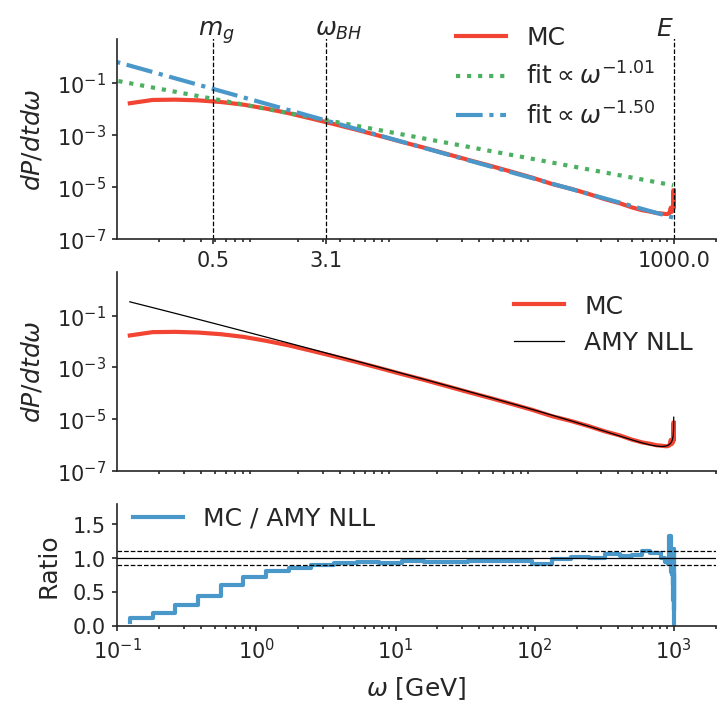
\includegraphics[width=.8\columnwidth]{spectrum.png}
}
\caption{The $q\rightarrow q+g$ splitting rate simulated in an infinite box with $T=0.5$ GeV. The quark energy is $E=1$ TeV. $\alpha_s = 0.1$. In the top plot, the spectrum $dR/d\omega$ (red line) is fitted to a power function $\omega^\lambda$ in different gluon energy regions. The green dashed line is fitted in the Bethe-Heitler region $\omega < \omega_{BH}\approx 2\pi T$; the blue dash-dotted line is fitted in the LPM region $\omega > \omega_{BH}$. The middle plot compares to the simulation to NLL solution to the AMY equation, and their ratio is shown in the bottom plot}
\label{fig:spectrum}
\end{figure}

In practice, to define a Monte-Carlo transport simulation an infinite medium limit and an eikonal limit of parton propagation, an ensemble of parton of certain species are initialized at a fixed energy $E_0$ and will be let propagate in the same direction.
Each time when a parton scatters elastically or splits, its splitting kinematics are taken down $\omega, k_\perp, t_0, \tau_f$, then the mother parton's energy is reset back to its initial value (a test in the eiknoal limit).
For elastic re-scatterings in the implementation of the LPM effect, the parton's energy is re-scaled back to the value before scatterings without changing its direction.
The system is evolved for a sufficiently long time $t_{\max}$, and only branchings that takes place within $[t_{\min}, t_{\max}]$ are analyzed to focus on the infinite time behavior of the simulation.

We start from the $q\rightarrow q+g$ channel.
The differential rate $dR/d\omega$ for a 1 TeV quark propagate through a medium of $T=0.5 GeV$ with coupling constant $\alpha_s = 0.1$ is shown in 
figure \ref{fig:spectrum}.
The vertical axis is the differential branching rate $dR/d\omega$, and the horizontal axis is the energy of the final state gluon $\omega$.
To better understand our result, we have put three ``landmark'' energy scales in the upper plot, which are the initial parton energy $E$, an estimate of the Bethe-Heitler energy $\omega_{\textrm{BH}}\sim\hat{q}_g \lambda_g^2 \sim 2\pi T$, and the screening mass $m_g = m_D/\sqrt{2}$.
In the LPM regime $\omega_{\textrm{BH}} < \omega$, the spectrum falls off as a power law with fitted exponent $-1.50$ (the blue dash-dotted line), and the in the Bethe-Heitler regime above the screening mass $m_g < \omega < \omega_{\textrm{BH}}$, the fitted power law exponent is close to $-1$ (the green dotted line).
These exponents are in good agreement with the theoretically expectation that $dR_{\textrm{BH}}/d\omega \propto \omega^{-1}$ and $dR_{\textrm{LPM}}/d\omega \propto \omega^{-3/2}$ from equations \ref{eq:incoh-dR} and \ref{eq:AMY-LL}.
The screening mass regulates the soft divergence of the spectrum below $m_g$.
One may notice a tiny increase of the spectrum when $\omega \rightarrow E$, this is region where the gluon takes a larger fraction of the initial quark's energy.

In the middle plot, we compare this result from simulation directly to the NLL solution of the AMY equation. 
As a remark, we have tuned the prefactor in the $b$-parameter to be $0.75$  by comparing to this theory prediction at $\alpha_s=0.1, E=1 \textrm{TeV}, T = 0.5 \textrm{GeV}$ for the $q\rightarrow q+g$ channel.
For the rest of the comparison with different coupling, parton energy, temperature, and channels, this parameter will {\bf not} be further tuned.
The simulation agrees with the NLL solution very well when $\omega \gg \omega_{\textrm{BH}}$ where the formula is valid.
The bottom plot show the ratio between the simulation and the theory, an level of $\pm 10\%$ agreement in the deep-LPM region is achieved in the static case.

\begin{figure}
\centering{
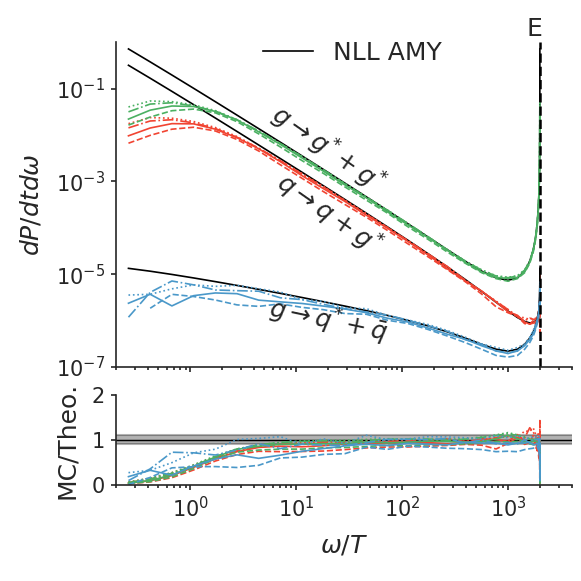
\includegraphics[width=.8\columnwidth]{channel_rate.png}
}
\caption{The rate of different channels $q\rightarrow q+g^*$, $g\rightarrow g+g^*$, and $g\rightarrow q^* + \bar{q}$ are plotted as functions of the daughter (labeled by "${}^*$") parton energy. The mother parton has a energy $E=1$ TeV. The medium temperature is $T=0.5$ GeV. $\alpha_s = 0.1$. The simulations (thick dashed lines) are compared to the NLL solutions (thin solid lines).}
\label{fig:channel_rate}
\end{figure}

Next, we would like to compare the simulation all the three channels in figure \ref{fig:channel_rate}.
The setup is the same as the figure \ref{fig:spectrum}.
The red, green and blue lines correspond to the differential branching rate of processes $q\rightarrow q+g^*$, $g\rightarrow g^*+g^*$ and $g\rightarrow q^*+\bar{q}$; the thin back lines are the NLL solution to the AMY equation.
The ``${}^*$'' sign denotes the final state parton whose energy is $\omega$.
For the case two final state gluons, both are taken into account in the simulation as they are identical particles.
We have discussed the feature the $q\rightarrow q+g$ in the previous paragraph. 
The spectrum shape of $g\rightarrow g+g$ process is very similar to the quark splitting channel in the range $\omega \ll E$, with a higher value.
The rate is symmetric with respect to $\omega = E/2$ due to its symmetric final states (though it is hard to tell from this double-log plot), so at large $\omega$, the rate goes up again.
The spectrum of $g\rightarrow q+\bar{q}$ is also symmetric with respect to $\omega = E/2$.
Though its final state consists of two different particle, the splitting function is still symmetric in this case.
We see that the simulation achieves a good agreement with the NLL solution in the deep-LPM region $\omega/T > 10$.

Next, we would like validate the simulation with different coupling constant and parton energies.
We choose both a relative small coupling $\alpha_s = 0.1 (g \approx 1.1)$ and a value closer to the phenomenology coupling $\alpha_s = 0.3 (g \approx 1.9)$, and vary the energy from $10$, $10^2$, to $10^3$ GeV.
The ratios between the simulation and the NLL solutions are shown in figure \ref{fig:sys-q2qg}, \ref{sys-g2gg} and \ref{fig:sys-g2qqbar}.
From these systematic comparison.
One see that the simulation reproduces the correct scaling in the LPM region, although due to the decreasing of the parton energy, this region also shrinks.
The overall performance of the modified Boltzmann transport in describing the inelastic processes in a large medium is good and under control.
One remaining problem is that the systematic deviation for the $g\rightarrow q+\bar{q}$ channel is bigger than the other two channels, as we did not include the backward region in its $2\rightarrow 3$ matrix-elements.

\begin{figure}
\centering
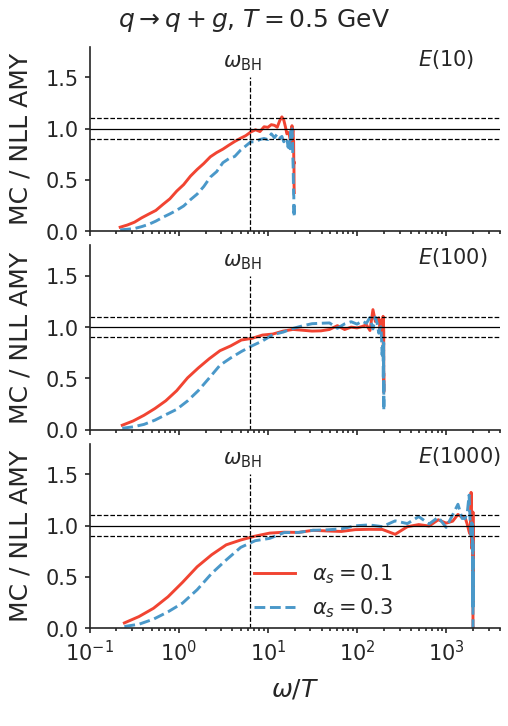
\includegraphics[width=.8\columnwidth]{spectrum_E_q2qg.png}
\caption{Ratios of splitting rate $dR/\omega$ between the modified Boltzmann simulation and the NLL solution for $q\rightarrow q+g$ splitting. The quark energies are $E$ is 10, 100, and 100 GeV from top to the bottom plot. 
And two coupling constants are used: $\alpha_s = 0.1$ (red solid lines) and $\alpha_s = 0.3$ (blue dashed lines).
$\omega$ stands for the gluon energy.
The horizontal dashed lines denote $\pm 10\%$ deviation from unity. }
\label{fig:sys-q2qg}
\end{figure}

\begin{figure}
\centering
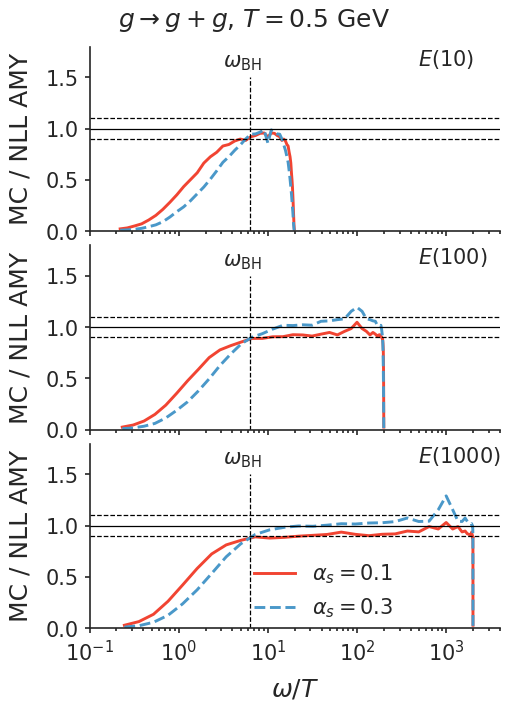
\includegraphics[width=.8\columnwidth]{spectrum_E_g2gg.png}
\caption{The same as figure \ref{fig:sys-q2qg}, but $g \rightarrow g + g$.}
\label{fig:sys-g2gg}
\end{figure}

\begin{figure}
\centering
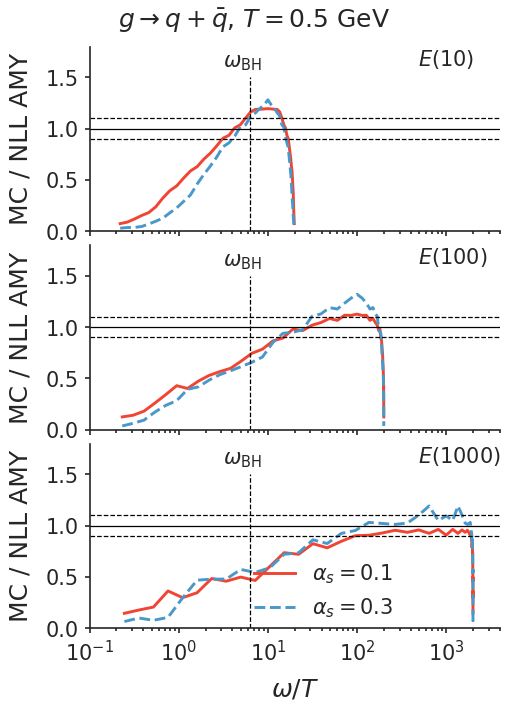
\includegraphics[width=.8\columnwidth]{spectrum_E_g2qqbar.png}
\caption{The same as figure \ref{fig:sys-q2qg}, but $g \rightarrow q + \bar{q}$.}
\label{fig:sys-g2qqbar}
\end{figure}

Finally, we validate the running coupling calculation in Fig. \ref{fig:running} using the $g\rightarrow g+g$ channel.
The theory curves (black lines) are obtained combining Eq. \ref{eq:AMY-LL} and Eq. \ref{eq:q3running}.
Different line styles correspond to the variation of the $Q_0$ value around an initial guess $m_D (E/T \ln(E/T) )^{1/4}$ by a factor of $2$ above and below.
For this 1 TeV parton, the scale $Q_0$ is actually very large and the running of $\alpha_s$ is rather slow, which explains the theory curve is not very sensitive to a factor of $4$ change in $Q_0$.
The simulation was performed using the running coupling prescription described in Section \ref{section:running}.
The overall shape of the spectrum in the deep LPM region is again well described by the modified Boltzmann simulation. 

\begin{figure}
\centering
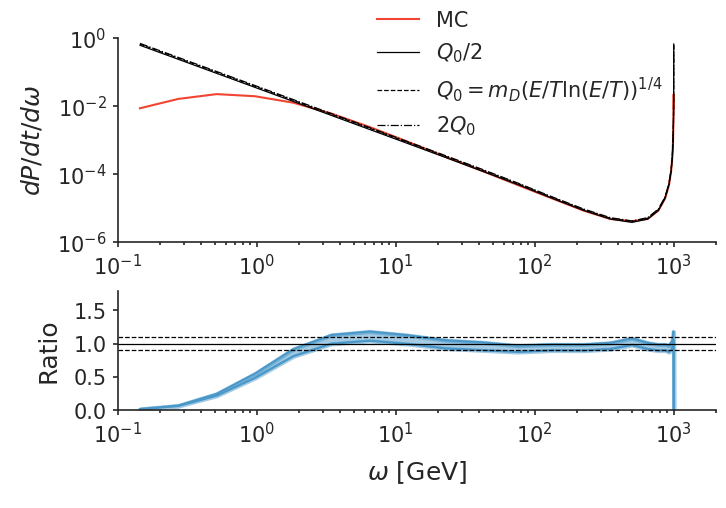
\includegraphics[width=.8\columnwidth]{running.png}
\caption{Comparing the simulation with running coupling constant the NLL solution with running $\alpha_s$ prescription.
The scale $Q$ in the emission vertex and in the theoretical formula for the effective transport parameter $\hat{q}_3$ (equation \ref{eq:q3running}) is chosen to be $1/2$, $1$ and $2$ times of the scale $\sqrt{\langle k_\perp^2\rangle}$ in equation \ref{eq:runscale}.
The ratio is shown in the bottom plot.}
\label{fig:running}
\end{figure}

\subsection{Branching in a finite / expanding medium}
We have made clear before that this approach is designed for interpolating the Bethe-Heitler region and the deep-LPM region in a large medium, and from the validation in the previous section, it indeed works very well.
However, the medium created in heavy-ion collisions were never in the large and static limit, its finite time and spatial extend, local hot spots fluctuations and the fast radial expansion can all make significant impact on the hard parton propagation. 
Therefore, we need to investigate how our approach would behave in a few more complex scenarios: a finite medium and and expanding medium, before applying such a model to phenomenological usage.

\paragraph{A semi-infinite medium}
Consider the semi-infinite medium with the static temperature profile,
\begin{eqnarray}
T = \begin{cases}
0 , z<0\\
T_0, z>0
\end{cases}
\end{eqnarray}
and hard partons are created at $z=0$ and propagate into the medium.
Deep inside the medium, the medium induced radiation should be getting asymptotically close to the calculation in an infinite medium.
At the boundary, there is a complicated interference between medium scatterings centers and the hard production vertex.
For a thin medium where the path length is short compared to the formation time, these interference terms can be worked out in the ``opacity expansion", or by analyzing the propagator in the path-integral formalism with the semi-infinite temperature profile.
This boundary effect results in a path length dependence of the medium induced branching rate that starts from zero at $t=0$ and gradually approach the asymptotic value in a large medium.
The resulting parton energy loss rate is significantly reduced due to this effect, and scales quadratic with the path length $\Delta E \propto L^2$ near the boundary and at larger times, it transits to $\Delta E \propto L$.

It is true that our approach is designed for a large medium, but it also displays certain finite size effect. 
Remember that the branchings in the modified transport approach takes a finite amount of time, and those branching that becomes independent at time $t$ are actually initiated by a $2\rightarrow 3$ processes at from a wide range of scattering centers in the past $t' = t - \tau_f$.
Therefore, if the medium is semi-infinite, and there were no scattering centers before $t' = t-\tau_f < 0$, then the medium-induced contribution to the branchings at time $t$ will be reduced.
This reduction gets weaker and weaker when the condition $t-\tau_f > 0$ can be satisfied by more and more induced branchings and eventually, when $t\gg \langle \tau_f\rangle$, this boundary effect dies off in the simulation. 
Of course, it is can not reach an quantitative level of agreement with the theory at $L \lesssim \tau_f$ since the interference pattern is not implemented.
We would like to check if this simulation boundary effect qualitatively mimic the interference physics that happens near the boundary.

\begin{figure}
\centering
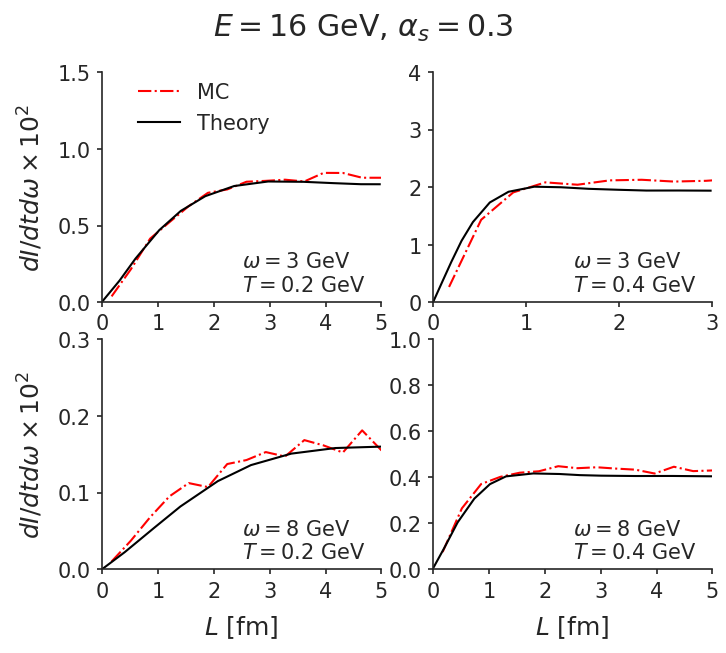
\includegraphics[width=.8\columnwidth]{spectrum_L.png}
\caption{The path-length dependence of the simulated $q\rightarrow q+g$ emission rate $dR/d\omega$ comapred to the direction calculation of formula \ref{eq:full-theory} from \cite{CaronHuot:2010bp}. $\alpha_s = 0.3$. The quark energy is $16$ GeV. The left and right columns have medium temperature $T=0.2$ and $0.4$ GeV respectively. The top and bottom rows show the differential rate at $\omega = 3$ and $8$ GeV.}
\label{fig:spectra-L-alphas=0.3}
\end{figure}

In Figure \ref{fig:spectra-L-alphas=0.3}, the differential rate obtained from simulation is compared to the numerical solution of the full leading order calculation for a finite medium.
The horizontal axis is the time of travel by the hard parton (path length divided by the speed of light), and each subplot shows how the branching rate changes as a function of time with different medium temperatures ($T=0.2$ GeV on the left, $T=0.5$ GeV on the right) and at different branching parton energy ($\omega=3$ GeV at the top, $\omega=8$ GeV at the bottom).
The theory curves are taken from the references \cite{CaronHuot:2010bp} for a 16 GeV parton with coupling constant $\alpha_s = 0.3$, and the red lines are our simulation.
The theory curve first increases linearly and then turn over to a constant value in the large medium limit for $t \gg \sqrt{2x(1-x)E/\hat{q}_3}$.
The simulation, as expected, reproduces the large time limit of the rate.
Moreover, we find that the current implementation also predicts the qualitative ``turn over'' of the spectra at finite path length.
The original paper only publish this calculation for a $16$ GeV quark. 
To validate if this qualitative agreement also holds at higher parton energies, we implement the numerical approach \cite{CaronHuot:2010bp} and compute the theoretical curves for $E=100$ GeV partons.
The comparison of simulation and numerical solutions are shown in figure \ref{fig:spectra-L-alphas=0.3-E100} and again, we found a qualitative agreement with the theoretical finite size effect.

\begin{figure}
\centering
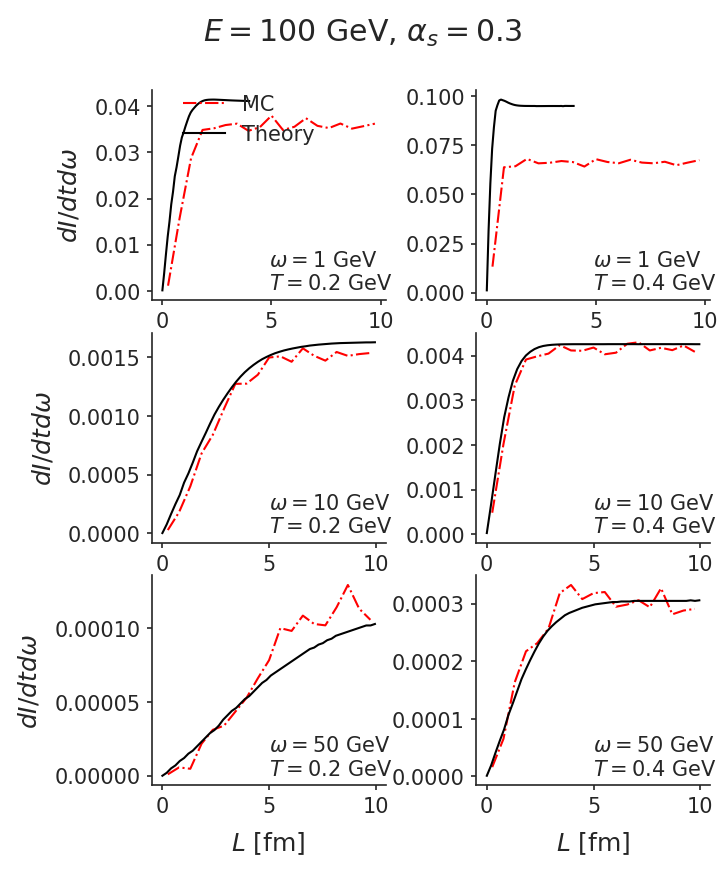
\includegraphics[width=.8\columnwidth]{spectrum_L_100.png}
\caption{The same as figure \ref{fig:spectra-L-alphas=0.3-E100}, but the initial quark energy is $100$ GeV, and is plotted for gluon at 5 (top), 10 (middle) and 50 (bottom) GeV.}
\label{fig:spectra-L-alphas=0.3-E100}
\end{figure}

\paragraph{An expanding medium}
Fast radial expansion is another important feature of the medium in heavy-ion collisions.
It causes the temperature to decrease drastically in the early stages of the expansion and introduces another time scale in which the medium temperature changes notably.
Assume a simplified power-law changing temperature profile
\begin{eqnarray}
T(\tau; \nu)^3 = T_0^3\left(\frac{\tau_0}{\tau}\right)^{2-1/\nu}.
\end{eqnarray}
The $\nu$ parameter controls the rate of expansion. 
$\nu = 1/2$ is the static medium limit, and $\nu=1$ is the Bjorken flow.
We can define the following medium expansion time, over which the transport parameter changes significantly,
\begin{eqnarray}
\tau_{\textrm{ex}} = \left(\frac{d\ln(T^3)}{d \tau} \right)^{-1} = \frac{\tau}{2-1/\nu}.
\end{eqnarray}
The larger the $\nu$ parameter is, the smaller the expansion time scale.
With $\tau_0 \sim 1$ fm/$c$, the expanding time scale can be short enough that energetic branchings already probes the changing temperature profiles within its formation time $\tau_f > \tau_{\textrm{ex}}$.
One consequences of this fast changing of temperature is that, for these branchings $\tau_f > \tau_{\textrm{ex}}$, the transition probability over a finite amount of time can not be well approximated by integrating rates that are calculated in an infinite box defined by the local temperatures,
\begin{eqnarray}
\frac{dP(t_1, t_2)}{d\omega} \neq \int_{t_1}^{t_2} \frac{dR_{\infty}(T(t))}{d\omega} dt,
\end{eqnarray}
where is the rate obtained by solving the branching rate in the infinite medium setup. 
This approach is employed in transport models like MARTINI and TEQULIA \cite{Jeon:2003gi,Schenke:2009gb,Dai:2019hbi}.
Our approach akes into account the changing of the medium temperature (and also flow velocity).
This is because the rescattering procedure that determines amount of suppression is performed along the trajectory of the hard partons and therefore naturally includes the effect of the cooling of the medium.
The typical formation time determined by the rescattering procedure is also changed by the expansion.
Recall that in a static medium the dimensionless combination that enters the leading-log formula is the $t/\tau_f \sim t \sqrt{\omega/\hat{q}}$, but with a $\hat{q}$ that is decreasing with temperature.
The self-consistent determination of the formation time requires the following relation to hold on average,
\begin{eqnarray}
t_2 - t_1 &=& \frac{2x(1-x)E}{k_{\perp}^2(t_1) + \int_{t_0}^{t} \hat{q}(\tau) d\tau},\\
\hat{q}(\tau) &=& \hat{q}(\tau_0) \left(\frac{\tau_0}{\tau}\right)^{2-1/\nu}
\end{eqnarray}
Neglecting the initial transverse momentum at $t=t_1$, we have the characteristic time scale $\Delta t = t_2 - t_1$ of this procedure in the expanding medium temperature profile as
\begin{eqnarray}
1 = \sqrt{\frac{\hat{q}(t_0)}{2x(1-x)E}} \tau_0 \sqrt{\frac{\nu-1}{\nu}} \left(\frac{\Delta t}{\tau_0}\right)^{1/2\nu}
\end{eqnarray}

\begin{figure}
\centering
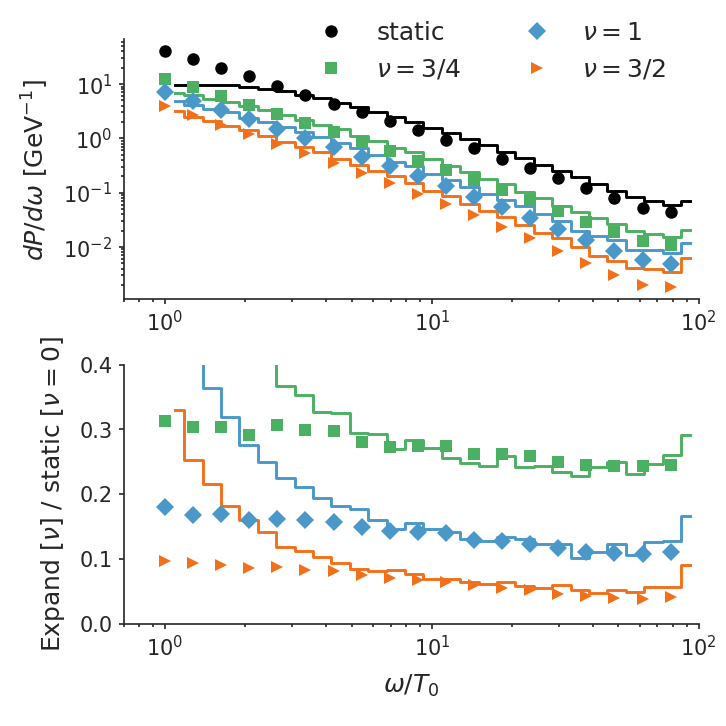
\includegraphics[width=.8\columnwidth]{spectrum_Bjorken.png}
\caption{Top plot: the simulated spectrum (diffusion plues diffusion-induced radiation only) using the parametric medium with expansion parameters $\nu = 0$ (static, black), $3/4$ (green), $1$ (Bjorken, blue), and $3/2$ (orange). The analytic results are shown in symbols and simulations in lines. $\alpha_s=0.3$. The expansion starts at $\tau_0 = 0.2$ fm/$c$ with an initial temperature $T_0 = 1$ GeV. Bottom plot: the ratios between calculation (simulation) in an expanding medium to that in the static medium.}
\label{fig:Bjorken-BDMPS}
\end{figure}

Making comparison to theoretical calculations, we make use of a result obtained in the BDMPS framework \cite{Baier:1996kr,Baier:1998yf}.
Using the power-law decreasing temperature profile, the obtained branching probability for the $q\rightarrow q+g$ splitting is \cite{Baier:1998yf},
\begin{eqnarray}
\frac{dP}{d\omega} &=& \frac{\alpha_s}{2\pi E}P_{q\rightarrow qg}(x)\mathfrak{Re}\int_{\tau_0}^{\tau_0+L}\frac{dt_f}{t_f}\int_{\tau_0}^{t_f}\frac{dt_i}{t_i} \frac{1}{\nu^2}\\
\nonumber
&& \left.\left[ I_{\nu-1}(z_i)K_{\nu-1}(z_f)-I_{\nu-1}(z_f)K_{\nu-1}(z_i)\right]^{-2}\right|_{\omega=xE}^{\omega=\infty},\\
z_{i,f} &=& 2i\nu \sqrt{\frac{\hat{q}_g(1-x+C_F/C_A x^2)}{2(1-x)\omega}} \tau_0 \left( \frac{t_{i,f}}{\tau_0}\right) ^{1/2\nu}.
\end{eqnarray}
This result goes back to the static BDMPS result \cite{Baier:1996kr} when $\nu=1/2$.
One potential problem of comparing the formula to our simulation is that this BDMPS calculation works in the multiple-soft limit (leading log).
Therefore, we used only the diffusion-induced radiation in the simulation and turned off the large-$Q$ $2\rightarrow 3$ scattering part.
Also as mentioned before, in the absence of the pertrubative tail in the collision kernel, $b=0.75$ is used without the logarithmic correcting factor in equation \ref{eq:NLL-b}.
In addition, we will not try to make a direct comparison of the spectra (top of figure \ref{fig:Bjorken-BDMPS}), but focusing more on the ratio between the expanding calculation/simulation over the static calculation/simulation instead (bottom of figure \ref{fig:Bjorken-BDMPS}).
This ratio reflects the change of the shape of the spectra due to the dropping of temperature.

The simulation uses a medium with initial temperature $T_0=1$ GeV at $\tau_0=0.2$ fm/$c$ and lasts until $\tau = 20$ fm/$c$ using four different expansion rate $\nu = 1/2, 3/4, 1, 3/2$.
These choice of numbers corresponds to a static medium, a slowly expanding medium, the Bjorken flow, and a faster-than-Bjorken expansion.
We found that when $\omega \gg T_0$, the degree of change in the radiation spectra is well reproduced by the modified transport simulations.

\begin{figure}
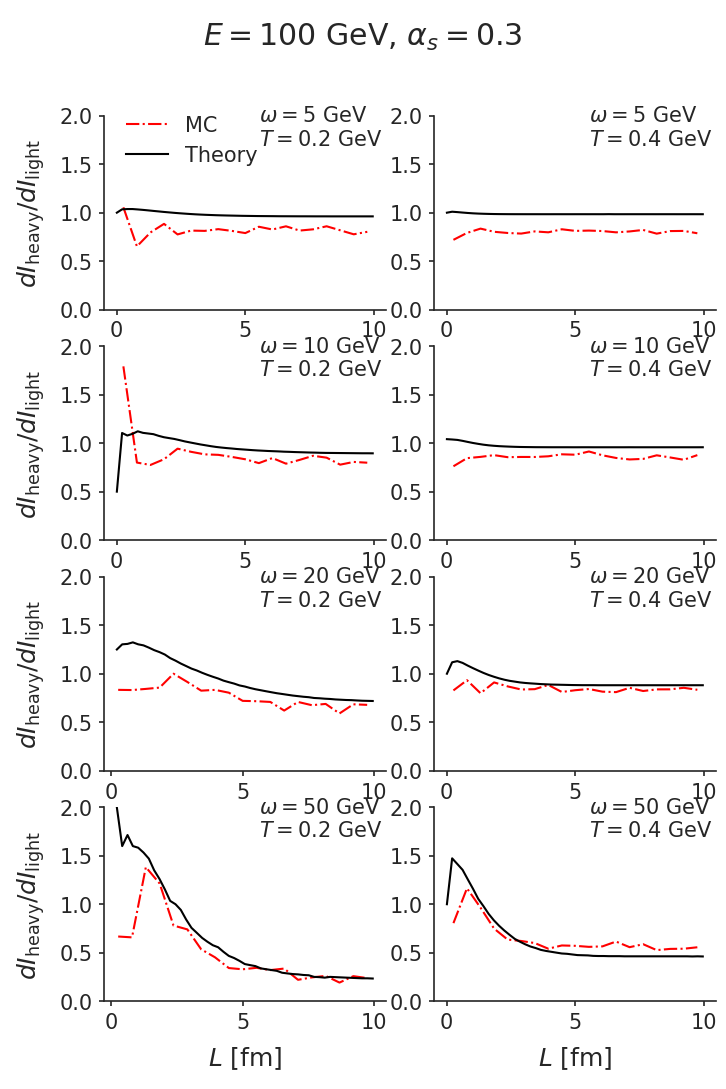
\includegraphics[width=\columnwidth]{mass.png}
\caption{The mass dependence of the radiation spectrum $q\rightarrow q+g$, presented as the ratio of bottom $dR/d\omega$ over the light quark $dR/d\omega$, as functions of path length. The left and right columns use temperatures 0.2 and 0.4 GeV. Different rows (from top to bottom) plot cases for gluon energy $\omega = 5, 10, 20, 50$ (GeV).}
\label{fig:mass}
\end{figure}

\subsection{Heavy quark and thermalization test}
Finally, we check the model performance for heavy quarks.
For short, to implement mass effect to the modified transport approach for inelastic scatterings, we use massive kinematics for the heavy quarks, include the mass term in the formation time, and implement the dead cone approximation after the transverse momentum is broadened by elastic collision.
The theory curves are obtained by solving the exact equation with a effective mass term,
\begin{eqnarray}
m_{\textrm{eff}}^2 = (1-x)m_g^2 + x^2 M^2
\end{eqnarray}
which includes both the thermal mass of the gluon and the current mass of the heavy quark.
We present the comparison between the simulation and the theory in terms of the ratio between the differential branching rate of the heavy quark (charm mass at 1.3 GeV, bottom mass at 4.2 GeV) and the light quark.
In figure \ref{fig:mass} for the bottom quark case, the horizontal axis is the path-length, and the vertical axis is the ratio.
Different rows take different radiated gluon energies, and different  columns has medium temperatures at $0.2$ GeV (left) and at $0.4$ GeV (right) respectively.
The initial bottom quark energy is 100 GeV and the coupling is $\alpha_s=0.3$.
We see that the dead-cone approximation better agrees with the theory calculation at larger $x$ and larger path-length.
Deviations observed at small path length is understand as the limitation of our implementation to the large medium, and should be better treated by the opacity expansion. 
The deviation at small $x$ is interesting, particularly, the theory almost predicts an identical heavy quark radiation spectra as the light quark. This absent of dead cone at small-$x$ is already observed in early works of heavy quark energy loss study in both the GLV framework and the BDMPS framework.
This means that the treatment of the mass effect is not as simple as the dead-cone approximation and should be improved in the future.


\paragraph{Thermalization of heavy quark}
\begin{figure}
\centering
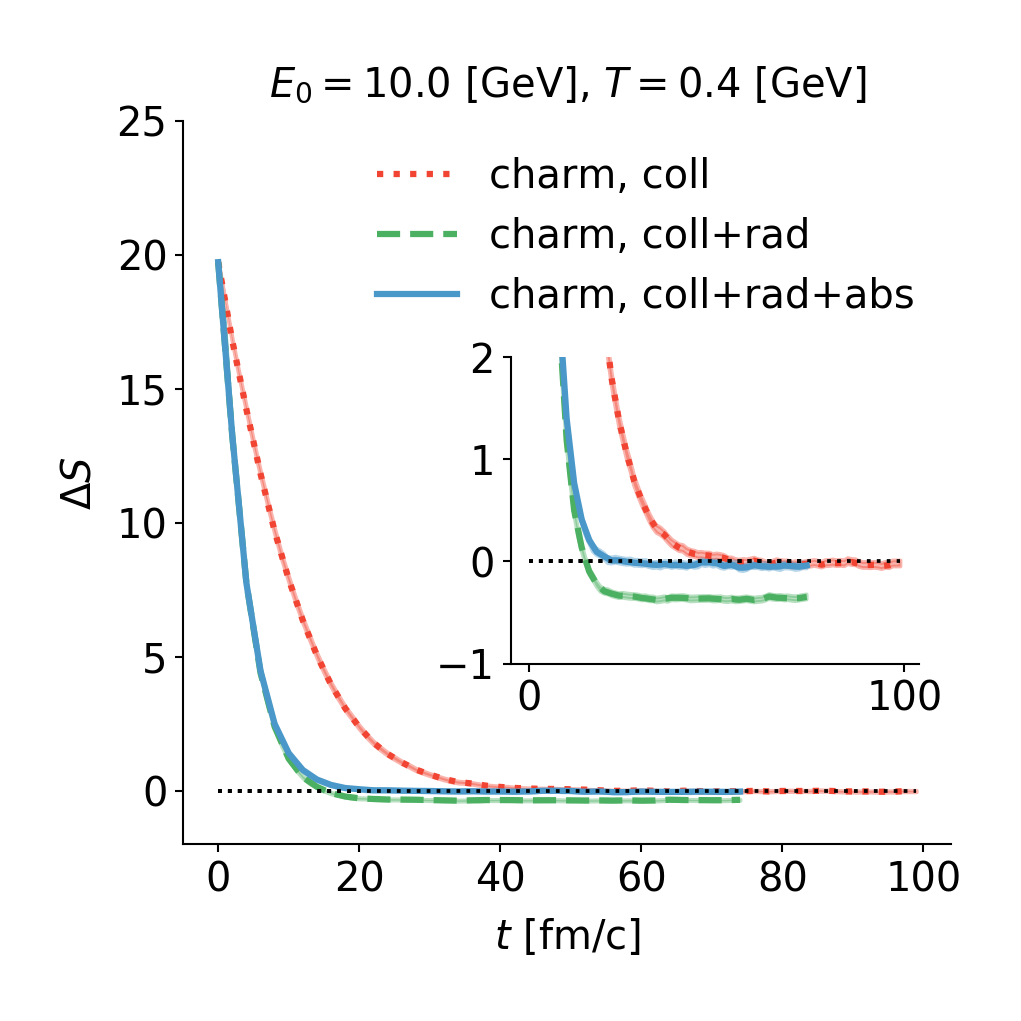
\includegraphics[width=.8\textwidth]{thermalization.png}
\caption{Approaching to thermal equilibrium of heavy flavor is quantified as the change of $\Delta S$ (defined in equation \ref{eq:DeltaS}) as function of time.. The red dotted lines includes elastic processes only. The green dashed line further includes $2\rightarrow 3$ and $1\rightarrow 2$ processes. The blue solid lines turn on the detailed balance processes $3\rightarrow 2$ and $2\rightarrow 1$.}
\label{fig:thermalization}
\end{figure}
Heavy quark's large mass made it takes longer time to thermalize and the low-$p_T$ end of the heavy quark production in the heavy-ion collision can carry the information non-equilibrium dynamics.
To extract the degrees of thermalization, one has to make sure the correct thermalized limited is achieved in the transport model, given enough time of evolution.
This is trivial for large-angle elastic scatterings and diffusion processes as long as the correct Einstein relation is imposed.
The $n\rightarrow n+1$ body radiative process is approximated by a initial $2\rightarrow 3$ or $1\rightarrow 2$ process and a sequence of elastic interactions; therefore, in principle the $n+1\rightarrow n$ absription processes need to be treated on the same footing to restore the detailed-balance in the modified-Boltzmann equation.
This can be done but is over complicated.
Here we argue that close to a few times of temperature, the LPM effect is not that strong that an incoherent implementation of the absorption is enough to study the bulk of particles close to thermal distribution.

We define a quantity $\Delta S$ to measure the approaching of thermal distribution $f_0 = e^{-E/T}$ of an ensemble of heavy quarks,
\begin{eqnarray}
\Delta S = - \langle \ln f_0 \rangle - S_0 \\
 &=& - \frac{1}{N}\sum_i\ln f_0(E_i) - \frac{\int dp^3 f_0 ln(f_0)}{\int dp^3 f_0}
 \label{eq:DeltaS}
\end{eqnarray}
Where the first term the the ensemble average of the the function $-\ln f_0$, and the subtracted term is proportional to the entropy of distribution $f_0$.
Note that the quantity is zero if the ensemble thermalize.
If the system is approaching thermal distribution with an effective temperature such that $f = e^{-E/T'}$, then $\Delta S$ is 
\begin{eqnarray}
\Delta S = \frac{\int dp^3 E/T e^{-E/T'}}{\int dp^3 e^{-E/T'}} - S_0 = \frac{T'-T}{T}
\end{eqnarray}
which is a measure of the deviation of the effective temperature from the thermal bath temperature.

Using this definition, we plotted $\Delta S$ as a function of time for 1000 heavy quark that are initialized at 10 GeV.
The temperature of the thermal bath is 0.5 GeV and we used a fixed $\alpha_s = 0.3$.
Under the influences of diffusion (red) and diffusion plus large-angle elastic collisions (green), $\Delta S$ decreases from a large value until fluctuating around zero after 25 fm/$c$ (red) and $15$ fm/$c$ (green).
Now, adding the radiative processes (blue), the $\Delta S$ reaches a value below zero, which is the false equilibrium.
Only after the balancing processes of parton absorption are also included (orange), the correct thermal equilibrium limit is restored. 
We also found that the absorption process only sets in when the ensemble is close enough to the thermal distribution, as the bue line and the orange line are almost overlapped until $\Delta S$ dropped to 0.3.
This is because the absorbed gluon follows the thermal distribution in the medium while phase-space for a high energy parton $E\gg T$ to absorb a low energy gluon is very limited $x<T/E$, compared to radiation processes where the value of $x$ is not restricted by the Boltzmann factor $e^{-xE/T}$.

\section{Comments on two other inelastic process implementations}
I find it beneficial to discuss two other inelastic processes implementations for reader's references. 
They are termed as the ``coherence factor" approach and the ``blocking radiation" approach.
I had used the previous approach in my earlier studies \cite{Ke:2018tsh}, but it is the problems I encountered in this method that later motivates the development of the ``modified Boltzmann transport'' method. 
I shall show in this section that in the deep-LPM region, the ``coherence factor" approach still qualitatively agrees with the power counting of the LPM suppression $\lambda_{el}/\tau_f$, though it only includes the effect of one medium scattering centers and the method can be logarithmic dependent on the infrared cut-off.
The ``blocking radiation'' approach, however,  does not reproduce the power counting of of the LPM suppression.
These two approach, together with the ``modified Boltzmann'' approach will be compared later using the ``energy loss" of a fixed energy quark.
First, we introduces these two other approaches.

\subsection{The coherence factor approach}
This approach is first implemented in the improved Langevin equation \cite{Cao:2013ita}, using the single medium-induced radiation probability from the higher-twist calculation \cite{Majumder:2009ge,Wang:2001ifa} and a prescription for multiple emissions.
The higher-twist formula of medium-induced radiation is derived for a high virtual parton, including the interference of the hard production vertex and one medium scattering center.
The single radiation rate reads,
\begin{eqnarray}
\frac{dN_g}{dx dk_\perp^2 dt} = \frac{\alpha_s P(x)\hat{q}_g}{\pi k_\perp^4} 2\left(1-\cos\frac{t-t_0}{\tau_f}\right), \tau_f = \frac{2x(1-x)E}{k_\perp^2}
\end{eqnarray}
Here the radiation rate is a time-dependent ($t$) one due to the interference with the hard production at time $t_i$. 
Note that the interference factor cancels the collinear divergence. 
The only divergence comes from soft emission $x\rightarrow 0$. 
This divergence is not a problem for computing more physical quantities such as the energy loss, as it will be balanced by the gluon absorption processes.
However, in order to apply rate formulation, an infrared cut-off $x>x_c$ has to be introduced. 

The advantage is that if there is only one radiation, then sampling the time dependent rate indeed reproduces the High-Twist calculation.
However, the ambiguity rises from the way it handles multiple emissions.
For example, one can compute the average number of emission by integrating this formula along the trajectory of the hard parton through and then samples the fluctuating number of emission with a Poisson distribution.
But of course, this would assume the parton energy is not significantly changed during the process, and it is not clear how the presence of more than one scattering center would change this picture.
Here we would like to discuss another method in dealing with multiple emission using the high twist formula in a time evolution manner \cite{Cao:2013ita}.
The algorithm goes as follows:
\begin{itemize}
\item[1.] Choose an infrared cut-off for the gluon energy $x_c \propto T/E$, and a small enough time step $\Delta t$, so that the average number of emission is much smaller than $1$ to suppress multiple emission within $\Delta t$,
\begin{eqnarray}
\langle N_g \rangle = \Delta t \int_{x_c}^1 dx \int dk_\perp^2 \frac{dN_g(t-t_0)}{dx dk_\perp^2 dt} \ll 1.
\end{eqnarray}
\item[2.] Sample N according to a Poisson distribution with $\langle N_g \rangle$. For $\langle N_g \rangle \ll 1$, it is sufficient to sample the two leading cases of $N=0, 1$, as the probability to have more than 1 emission is negligible ($P_{N>2} = 1-e^{-\langle N_g \rangle}-e^{-\langle N_g \rangle}/\langle N_g \rangle = O(\langle N_g \rangle^2) \ll P_1 \ll P_0$).
\item[3.] If $N=0$ then propagate the parton to the $t+\Delta t$. If $N=1$, then sample the emission gluon's $x$, and $\vec{k_\perp}$ by the differential rate. {\it Meanwhile, $t_0$ is set to $t$}, so that the next emission's probability will accumulated from zero again.
\item[4.] Proceed for the next time step.
\end{itemize}
We found that the key step here is resetting the clock $t_0 = t$ for the parton after every emission.
As a result, from the second emission, the time difference that appears in the interference factor $t-t_0$ are the one measuring between two medium scattering centers.
Therefore, we will not interpret this procedure as the high-twist rate (interference between initial hard vertex and one medium collision center) starting from the second emission;
instead we understand it as an ansatz, from the second emission, to treat medium-induced emission in a large medium, as it do not require any information to the production vertex.

Considering it only includes one medium scattering center in the trigger the radiation, one wonders if this approach reproduces any in-medium radiation features predicted by the theory.
It is not immediately clear that what this iterative procedure predicts  expect through simulations. 
But if one pondering on the meaning of the ``clock resetting" step, then the typical $\Delta = t-t_0$ between two emissions are a time scale within which the emission probability reaches order one,
\begin{eqnarray}
1 \sim \int_{t_0}^{t} dt\int_{x_c}^1 dx \int dk_\perp^2 \frac{dN_g(t-t_0)}{dx dk_\perp^2 dt}.
\end{eqnarray}
With this key observation, after a few step of algebra, we are able to learn the qualitative feature of this approach.
Taking the soft approximation $P(x) \sim 2/x$, $\tau_f\sim 2xE/k_\perp^2$, and perform the time integral first, then the $k_\perp$ integral with limits from $0$ to $xE$.
\begin{eqnarray}
1 &\sim& 4\alpha_s\hat{q}\Delta t \int_{x_c}^1 \frac{dx}{x} \int \frac{dk_\perp^2}{k_\perp^4}\left(1-\frac{\sin(\Delta t/\tau_f)}{\Delta t/\tau_f}\right)\\
&=& \alpha_s\hat{q}_g \Delta t^3 \int_{\frac{\Delta t E x_c}{2}}^{\frac{\Delta t E}{2}} 
\frac{du}{u^2} \frac{u^2 \mathrm{Si}(u) -2u + \sin(u) + u\cos(u)}{u^2}\\
&=& \frac{\alpha_s\hat{q}_g \Delta t^3}{3u^3} \left(
u^3\mathrm{Ci}(u)-3u^2\mathrm{Si}(u) \right.\\\nonumber
&&\left.\left.- u^2 \sin(u) +3u-\sin(u) - 2u\cos(u)\right)\right|_{\frac{\Delta t E x_c}{2}}^{\frac{\Delta t E}{2}} 
\end{eqnarray}
This final integral of $x$ (reparametrize by $u = xE\Delta t/2$) would have been logarithmic divergent if we had not cut it at $x_c$ at the lower bound.
The result has the following expansion at small $u$: $\frac{1}{18}(6\ln(u)+6\gamma_E - 17)$ and decay to $0$ at infinite therefore a good proxy is to use the small-$u$ expansion but cut-off the upper bound of $u$ at its zero, and finally
\begin{eqnarray}
1 &\sim&  \frac{\alpha_s\hat{q}\Delta t^3}{3}\ln\frac{2}{ x_c E \Delta t } \propto (g^2 T \Delta t)^3 \ln\frac{2}{ x_c E \Delta t }
\end{eqnarray}
Now, it is clear that this procedure of implementing multiple emission inside the medium resets the clock in the interference factor every $1/g^2T$ up to certain logarithm dependence on the infrared cut-off, which is the order of the elastic collision mean-free-path.
Put this estimated $\Delta t$ back into the interference factor $2(1-\cos(\Delta t/\tau_f))$, one indeed find that the radiation spectrum will be strongly suppressed if the formation time is much greater than $\Delta t\sim \lambda_{el}$.

This suppression certainly mimic some property of the in-medium LPM effect, but is introduced by a very different mechanism.
Remember that the LPM effect is the suppression of single particle emission rate through multiple collision with the medium, without any information about how subsequent emissions are correlated. 
While the interference factor approach mimic the effect of the LPM suppression through correlation between subsequent emissions.
This will introduce several problems: 
\begin{itemize}
\item[1.] The correlation between subsequent emissions is in fact physics beyond leading order and requires new type of diagrams to be computed.
\item[2.] As we have seen, this procedure is affected by the choice of the infrared cut-off. Though its dependence is very weak, it is still a dependence that we try to avoid.
\end{itemize}

\subsection{The ``blocking radiation'' approach}
This is another approach we found in the literature \cite{ColemanSmith:2012vr}.
I would like to show that this approach is more problematic than the previous one, because it suppresses radiation with $\tau_f > \lambda_{\textrm{inel}}^{\textrm{incoh}}$ but not $\tau_f > \lambda_{\textrm{el}}$.

In this approach, the splitting is also first generated through an incoherent processes at time $t_0$, and then the self-consistently determination the formation time by elastic broadening. 
But its LPM suppression is introduced by requiring no other radiation is allowed from this radiator within the time from $t_0$ to $t_0 + \tau_f$.
This clearly introduces a correlation between subsequent emission, while the LPM effect concerns only the one particle emission rate.
While in our approach, the suppression is implemented by accepting the process with probability $\sim \lambda_{el}/\tau_f$, and more importantly, other emissions are unaffected by the current ``imaginary splitting" as most of them would be rejected without causing any physical effect.

A closer investigation reveals bigger problem.
Moreover, this ``blocking radiation" approach effectively reduces every $\tau_f/\lambda_{inel}$ incoherent emission to one, resulting only an overall reduction in the radiation spectrum without changing its shape.
And the suppression factor $\lambda_{inel}/\tau_f$ is different from the expected one, this is in fact an order of $\alpha_s$ wrong as the mean-free-path of the incoherent radiation rate contains one more power of $\alpha_s$ than $\lambda_{el}$.

\begin{figure}
\centering
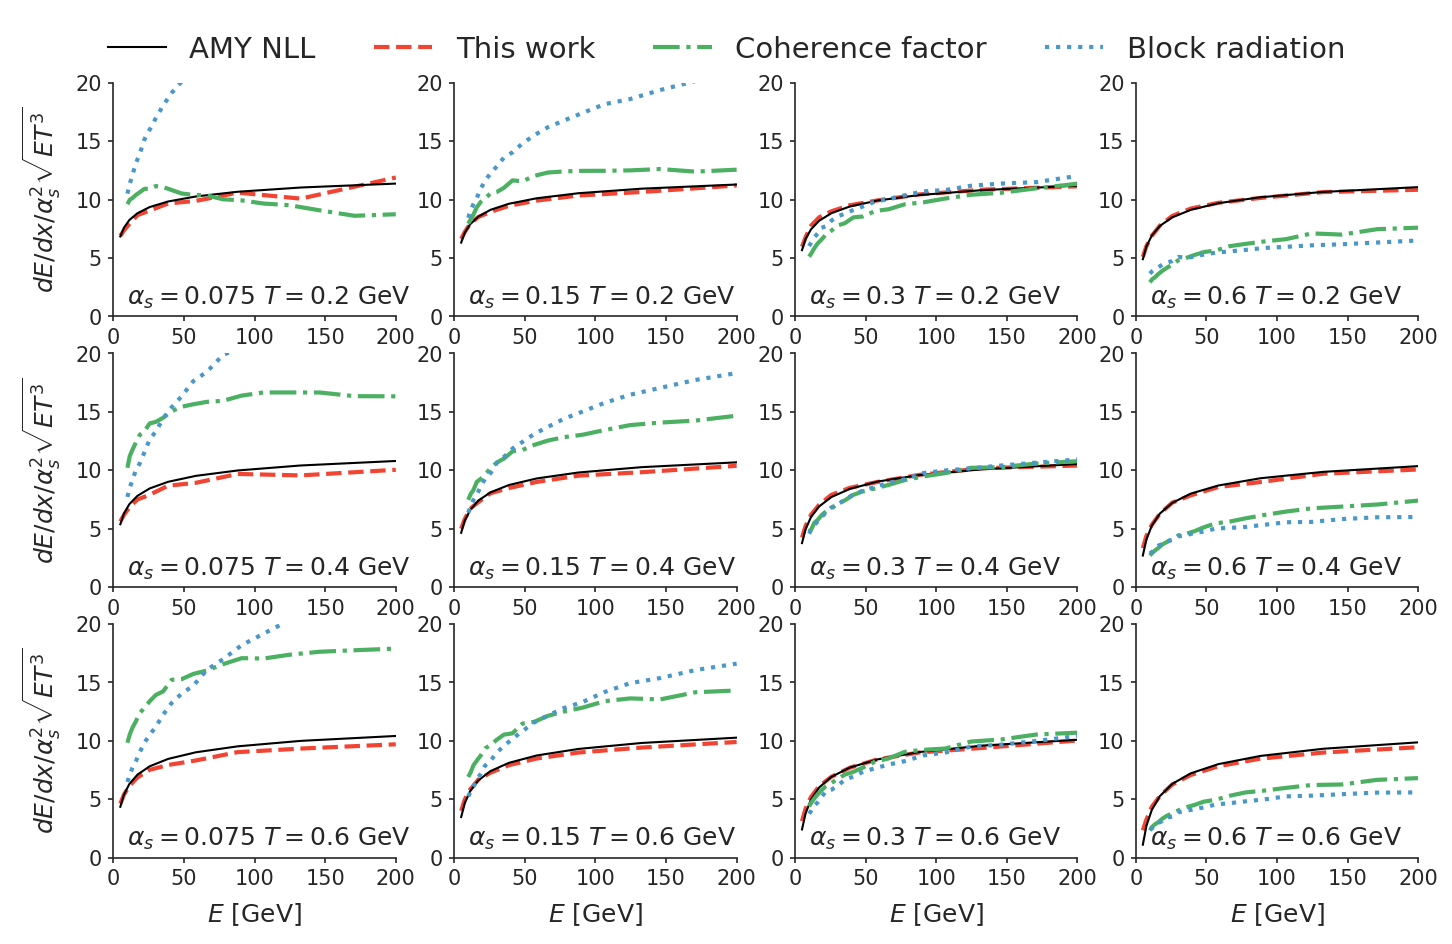
\includegraphics[width=1.\textwidth]{Eloss_infinite.png}
\caption{Energy loss per unit path lengh $dE/dx$ as a function of energy $E$, temperature $T$ and coupling constant $\alpha_s$. Each column corresponds to a value of the coupling constant $\alpha_s = 0.075, 0.15, 0.3$, and $0.6$ (from left to right). Each row corresponds to a temperature of $T = 0.2, 0.4$, and $0.6$ GeV (from top to bottom). $dE/dx$ is divided by the expected scaling $\alpha_s^2 \sqrt{ET^3}$. The MC implementations in this work (red dashed lines) is compared to the ``coherence factor" approach (green dash-dotted lines) and the ``block radiation" approach (blue dotted lines). The analytic results are denoted as black solid lines.}
\label{fig:eloss-inf}
\end{figure}

\begin{figure}
\centering
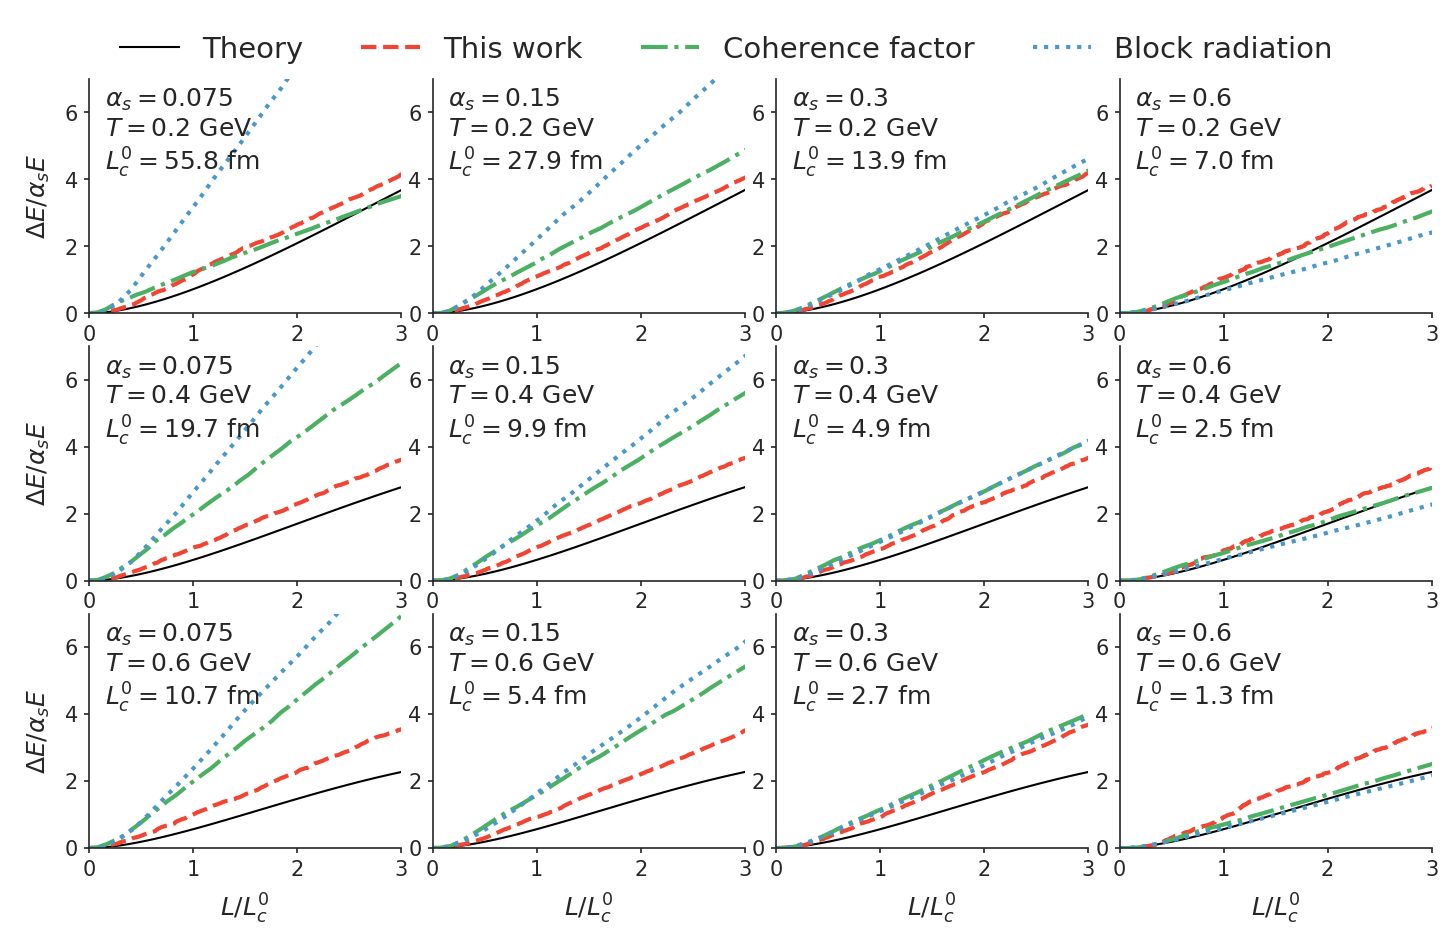
\includegraphics[width=1.\textwidth]{Eloss_Ldep.png}
\caption{Energy loss $\Delta E$ as a function of path length $L$, temperature $T$ and coupling constant $\alpha_s$. Each column corresponds to a coupling constant of value $\alpha_s = 0.075, 0.15, 0.3$, and $0.6$ (from left to right). Each row corresponds to a temperature of value $T = 0.2, 0.4$, and $0.6$ GeV (from top to bottom). $\Delta E$ is scaled by $\alpha_s E$ and $L$ is scaled by an estimated critical path length $L_c^0 = \sqrt{E/\hat{q}_0}$, $\hat{q}_0 = C_A \alpha_s T m_D^2$. The MC implementations in this work (red dashed lines) is compared to the ``coherence factor" approach (green dash-dotted lines) and the ``block radiation" approach (blue dotted lines). The analytic results for a thin medium are denoted as black solid lines.}
\label{fig:eloss-ldep}
\end{figure}

\subsection{Energy loss comparison among the three approaches}
In Figure \ref{fig:eloss-inf}, we show the calculation of energy loss per unit path length $dE/dx$ of a quark in an ``infinitely large" medium. 
Technically, $dE/dx$ is measured after an evolution time long enough ($L\gg L_c$) that finite size effects have faded away.
The results presented are normalized by $1/(\alpha_s^2 \sqrt{ET^3})$ in anticipation of the scaling $dE/dx \propto \alpha_s^2 \sqrt{ET^3}$.
For each column, we double the value of $\alpha_s$ and for each row, the temperature is increased by $0.2$ GeV. 
Within each subplot, the parton energy varies from $10$ GeV to $200$ GeV.
Different Monte Carlo implementations of the LPM effect are shown in colored lines, AMY NLL results are shown as black bands (we only integrate $\omega$ above the the Debye mass to calculate the AMY energy loss). 
Without a surprise, the ``modified approach" approach (red-dashed lines) reproduces the energy, temperature, and coupling constant dependence of AMY NLL energy loss very well.
The ``coherence factor" approach (blue-dash-dotted lines) has a similar energy and temperature dependence to that of the theoretical baseline; however, it systematically deviates from the baseline for different values of the coupling constant in a logarithmic manner.
For the ``block radiation" approaches, the deviations from the baseline regarding their $\alpha_s$-dependence are even bigger and the energy dependence also gets worse, which is not surprising as we have discussed its problem.

Next we examine the path-length ($L$) dependence of the energy loss $\Delta E$ of a quark with an initial energy of $E = 200$ GeV in a finite medium in Figure \ref{fig:eloss-ldep}.
Again, each column uses a different coupling constant and each row uses a different temperature. 
The path length within each subplot is varied up to four times $L_c^0$.
Here $L_c^0 = \sqrt{E/\hat{q}_0}$ with $\hat{q}_0 = C_A \alpha_s T m_D^2$ estimating the critical path length below which one expects a clear non-linear path-length dependence.
All three implementations show the non-linear increase of $\Delta E$ as function of $L$.
The ``modified Boltzmann" approach stays close to the theory calculations when $L<L_c^0$ for all cases, while the other two approaches deviate systematically as $\alpha_s$ is varied, similar to our previous findings for the energy-loss in the infinite matter case.

\section{Few-body matrix-elements}
\label{transport:ME}
This section provides the detailed $2\leftrightarrow 2$ and $2\leftrightarrow 3$ matrix-elements we used in the transport model.
The $2\leftrightarrow 2$ results are standard and we do not re-derive here.
The $2\leftrightarrow 3$ cross-sections are more complicated and a detailed derivation is attached to show the approximations we made for readers reference.

\subsection{$2\leftrightarrow 2$ processes}
The two-body scatterings between quarks, anti-quarks and gluons are standard and we quote the results from existing references \cite{RevModPhys.59.465}.
For a light parton scattering, we keep only $\hat{t}$-channel contribution, the $\hat{s}$ and $\hat{u}$ channel contribution are suppressed at high energy.
\begin{eqnarray}
\overline{|M_{q_1q_2\rightarrow q_1q_2}|^2} &=& \frac{64\pi^2 \alpha_s^2}{9} \frac{s^2+u^2}{t^2} \\
\overline{|M_{gg\rightarrow gg}|^2} &\approx& 72\pi^2 \alpha_s^2 \frac{-su}{t^2}
 \\
\overline{|M_{qg\rightarrow qg}|^2} &\approx& 16\pi^2 \alpha_s^2 \frac{s^2+u^2}{t^2}
\end{eqnarray}
For the heavy quark, since we are interested in its diffusion dynamics at low $p_T$, we uses the exact leading order matrix-element in the vacuum.
\begin{eqnarray}
\overline{|M_{Qq\rightarrow Qq}|^2} &=& \frac{64\pi^2\alpha_s^2}{9} \frac{(M^2-u)^2 + (s-M^2)^2 + 2 M^2 t}{t^2}
\nonumber
\\
\overline{|M_{Qq\rightarrow Qq}|^2} &=& \pi^2 \left\{
32\alpha_s^2 \frac{(s-M^2)(M^2-u)}{t^2} \right.
\nonumber
\\
&+&\frac{64}{9}\alpha_s^2 \frac{(s-M^2)(M^2-u)+2M^2(s+M^2)}{(s-M^2)^2} \nonumber
\\
&+&\frac{64}{9}\alpha_s^2 \frac{(s-M^2)(M^2-u)+2M^2(u+M^2)}{(M^2-u)^2} \nonumber
\\
&+& \frac{16}{9}\alpha_s^2 \frac{M^2(4M^2 - t)}{(M^2-u)(s-M^2)} 
\nonumber
\\
&+& 16 \alpha_s^2 \frac{(s-M^2)(M^2-u)+M^2(s-u)}{t(s-M^2)}
\nonumber
\\
&-& \left. 16 \alpha_s^2 \frac{(s-M^2)(M^2-u)-M^2(s-u)}{t(M^2-u)}\right\}
\end{eqnarray}

\begin{figure}
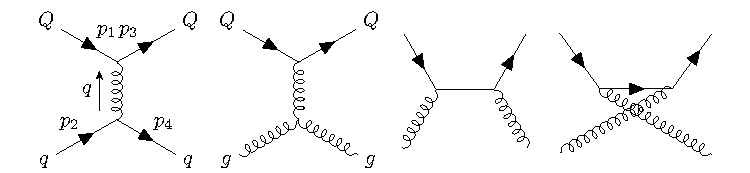
\includegraphics[width=\textwidth]{feyn-el.pdf}
\caption{Elastic processes: The first diagram corresponds to heavy quark ($Q$) - light quark ($q$, $\bar{q}$) scattering. The last three diagrams contribute to heavy quark ($Q$) - gluon ($g$) scattering.}\label{plots:feyn-elastic}
\end{figure}

\subsection{$2\rightarrow 3$ matrix-elements}
Large-Q $2\rightarrow 3$ inelastic processes are $g + i \rightarrow q+\bar{q} + i$, $q+i\rightarrow q+g+i$ and $g+i\rightarrow g+g+i$, where $i$ stands for a medium parton, and the rest symbols stands for hard parton.
In medium frame, hard parton has an energy $E\gg T$, while the medium thermal parton has $E\sim T$, and the typical center-of-mass energy is therefore $\sqrt{6ET}$.
We perform the calculation in the the center-of-mass frame of the two incoming parton and let the hard parton to be moving towards the $+z$ direction with momentum $p_1$, and the medium parton moving to the $-z$ direction with $p_2$.
The hard parton then splits into two daughter partons with momenta $k$ and $p_1 + q - k$.
The momentum transfer $q$ between the hard parton and the medium parton is thought to be large enough $|q| > Q_{\textrm{cut}}$ so we neglect the thermal correction to its propagator.

Our derivation largely follows the work \cite{Fochler:2013epa} while relaxing the soft approximation $xq_\perp \ll k_\perp$ in \cite{Fochler:2013epa}, and we only use the collinear approximation $k_\perp^2, q_\perp^2 \ll x(1-x) \hat{s}$ with $x = k^+/\sqrt{s} = k_\perp e^y_k /\sqrt{s}$.
Also, we only include the contributions with a $\hat{t}$-channel momentum exchange between the medium and the hard partons.
The collinear approximation requires $y_k \gg \ln(k_\perp/\sqrt{s})$ so that $y_k$ cannot be arbitrarily small and $y_k>0>\gg -\ln(\sqrt{s}/k_\perp)$ is a reasonable range of application.
Because $\hat{s}\sim 6 ET$, we expect this approximation to break down when either the typical values of $q_\perp^2$ becomes comparable to $x(1-x)6ET$ or when $y_k<0$ ($x < k_\perp/\sqrt{s} \sim k_\perp/\sqrt{6ET}$).
We shall briefly mention the treatment of the $y_k<0$ region in the end.

The light-cone momentum for $p_1$ , $p_2$ and $k$ can written down directly using $\sqrt{s}$, $x$ and $k_\perp$, then applying the above collinear condition, the expression for $q$ (and therefore $p_3$ and $p_4$) is obtained by kinematic constraint up to corrections of order $\{k_\perp, q_\perp^2\}/x(1-x)\hat{s}$.
\begin{eqnarray}
p_1 &=& (\sqrt{s}, 0, \vec{0})\\
p_2 &=& (0, \sqrt{s}, \vec{0})\\
k &=& (x\sqrt{s}, \frac{k_\perp^2}{x\sqrt{s}}, \vec{k}_\perp)\\
q &\sim& (-\frac{q_\perp^2}{\sqrt{s}}, \frac{q_\perp^2 + k_\perp^2/x - 
2\vec{q}_\perp \cdot \vec{k}_\perp}{(1-x)\sqrt{s}}, \vec{k}_\perp)
\end{eqnarray}
Using the light-cone gauge with a light-like vector $n = (0, 1, 0)$, the gauge fixing condition $n\cdot A =0$ eliminates the ``+" component in the gluon (with momentum $p$) polarization vector, and is obtained by applying the transverse condition $\epsilon \cdot p = 0$ (up to a higher order correction to its normalization)
\begin{eqnarray}
\epsilon(p) &\sim& (0, \frac{2\vec{\epsilon}_\perp\cdot\vec{p}_\perp}{p^+}, \vec{\epsilon}_\perp).
\end{eqnarray}
With these preparations, the matrix-element is factorized into an amplitude for the splitting process (approximated in the collinear limit) times the amplitude for two-body collision with the medium parton.
We shall only derive explicitly the cases where the medium parton is a quark, for colliding with medium anti-quark and gluon, it is sufficient to replace the $H+q\xrightarrow{\hat{t}} H+q$ amplitude by $H+\bar{q}\xrightarrow{\hat{t}} H+\bar{q}$ and $H+g\xrightarrow{\hat{t}} H+g$.
The connect of these results to the Bethe-Heitler limit of the AMY integral equation will be elucidated in the end.

\paragraph*{Gluon splitting to quark-anti-quark pair}
\begin{figure}
\centering
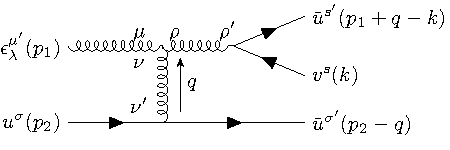
\includegraphics[width=.5\textwidth]{Large-Q-g2qqbar-A.pdf}\\
\vspace{1em}
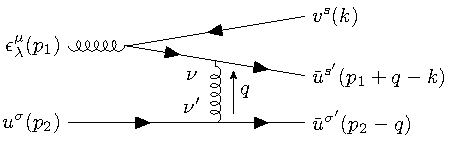
\includegraphics[width=.49\textwidth]{Large-Q-g2qqbar-B.pdf}\hfill
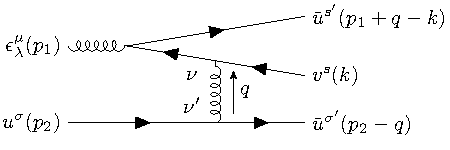
\includegraphics[width=.49\textwidth]{Large-Q-g2qqbar-C.pdf}
\caption{Three diagrams $A$ (Top), $B$ (Bottom left), $C$ (Bottom right) that contribute to the large angle scattering induced gluon splitting into quark-anti-quark pair in the forward region of the center-of-mass frame.}
\label{fig:feyn-g2qqbar}
\end{figure}

Three Feynman diagrams contribute to the kinematic region $y_k >0$ in the current approximation, as shown in figure \ref{fig:feyn-g2qqbar}.
We start from the amplitude for diagram $A$.
\begin{eqnarray}
i M_A &=& (-ig)^2(-g)f^{abc}(t^b)_{j'j}(t^c)_{i'i} \epsilon_\lambda^\mu(p_1) \\\nonumber
&&\frac{-i}{(p_1+q)^2}\left(g^{\rho\rho'}-\frac{n^{\rho}(p_1+q)^{\rho'}+n^{\rho'}(p_1+q)^\rho}{n\cdot (p_1+q)}\right) \bar{u}^s(p_1+q-k)\gamma_{\rho'}v^{s'}(k) \\ \nonumber
&&\frac{-i}{q^2}\left(g^{\nu\nu'}-\frac{n^{\nu}q^{\nu'}+n^{\nu'}q^\nu}{n\cdot q}\right) \bar{u}^{\sigma}(p_4)\gamma_{\nu'}u^{\sigma'}(p_2) \\ \nonumber
&& \left[g_{\mu\nu}(p_1-q)_\rho + g_{\nu\rho}(2q+p_1)_\rho + g_{\rho\mu}(-2p_1 -q)_\nu \right]
\end{eqnarray}
Next, express the projection matrix of the gluon propagator with momentum $p_1+q$ by the sum of tensor products of its polarization vectors, and identify the amplitude $iP_{A,\lambda'}^{ss'}$ for a gluon with polarization $\lambda'$ to split into the quark and anti-quark pair with spin $s$ and $s'$.
Also, use the high energy approximation to replace $\bar{u}^i(a)\gamma^\alpha u^j(b)$ by $(a+b)^\alpha \delta^{ij}$, then
\begin{eqnarray}
i M_A &\approx& -g^3 f^{abc}(t^b)_{j'j}(t^c)_{i'i} \delta^{\sigma\sigma'} \epsilon^\mu(p_1) \\\nonumber
&&\frac{1}{(p_1+q)^2} \sum_{\lambda'=\pm}\epsilon_{\lambda'}^{\rho}(p_1+q)\underbrace{\epsilon_{\lambda'}^{*,\rho'}(p_1+q) \bar{u}^s(p_1+q-k)\gamma_{\rho'}v^{s'}(k)}_{iP_{A,\lambda'}^{ss'}} \\ \nonumber
&&\frac{1}{q_\perp^2}\left(g^{\nu\nu'}-\frac{n^{\nu}q^{\nu'}+n^{\nu'}q^\nu}{n\cdot q}\right) (2p_2-q)_{\nu'} \\ \nonumber
&& \left[g_{\mu\nu}(p_1-q)_\rho + g_{\nu\rho}(2q+p_1)_\rho + g_{\rho\mu}(-2p_1 -q)_\nu \right] \\
&=& -g^3 f^{abc}(t^b)_{j'j}(t^c)_{i'i} \frac{1}{(p_1+q)^2}\frac{1}{q_\perp^2} \sum_{\lambda'=\pm}iP_{A,\lambda}^{ss'} \delta^{\sigma\sigma'}  \\ \nonumber
&& \epsilon_\lambda^\mu(p_1)2p_2^{\nu} \epsilon_{\lambda'}^{\rho}(p_1+q) \left[g_{\mu\nu}(p_1-q)_\rho + g_{\nu\rho}(2q+p_1)_\rho + g_{\rho\mu}(-2p_1 -q)_\nu \right].
\end{eqnarray}
Finally, we evaluate the contraction in the second line using the expression for $p_1, q$ and $\epsilon$, and keep only terms that is leading in $q_\perp^2/s$ to get,
\begin{eqnarray}
i M_A \approx -g^3 f^{abc}(t^b)_{j'j}(t^c)_{i'i}\delta^{\sigma\sigma'}\frac{2s}{q_\perp^2} \frac{x(1-x)}{(\vec{k}_\perp-x \vec{q}_\perp)^2} iP_{A,\lambda}^{ss'}.
\end{eqnarray}

Diagram B and C are similar and we only write down diagram B in detail.
\begin{eqnarray}
i M_B &=& (-ig)^3 (t^bt^a)_{i'i}(t^b)_{j'j} \epsilon_\lambda^\mu(p_1) \\\nonumber
&&\frac{-i}{q^2}\left(g^{\nu\nu'}-\frac{n^{\nu}q^{\nu'}+n^{\nu'}q^\nu}{n\cdot q}\right) \\\nonumber
&&\bar{u}^s(p_1+q-k)\gamma_{\nu}\frac{i(\slashed{p_1}-\slashed{k})}{(p_1-k)^2}\gamma^{\mu}v^{s'}(k) \\ \nonumber
&&\bar{u}^{\sigma}(p_4)\gamma_{\nu'}u^{\sigma'}(p_2)
\end{eqnarray}
Again, represent the tensor structure of the fermion propagator by the sum of tensor products of the spinors, identify the splitting amplitude $iP_{B,\lambda'}^{ss'}$ and use the high energy limit of the current,
\begin{eqnarray}
i M_B &\approx& ig^3 (t^bt^a)_{i'i}(t^b)_{j'j}  \\\nonumber
&&\frac{-i}{q_\perp^2}\left(g^{\nu\nu'}-\frac{n^{\nu}q^{\nu'}+n^{\nu'}q^\nu}{n\cdot q}\right) (2p_2-q)_\nu' \\\nonumber
&&\frac{1}{2p_1\cdot k} \sum_\sigma \bar{u}^s(p_1+q-k)\gamma_{\nu} u^{\sigma}(p_1-k) \underbrace{\epsilon_\lambda^\mu(p_1)\bar{u}^{\sigma}(p_1-k) \gamma^{\mu}v^{s'}(k)}_{iP_{B,\lambda}^{\sigma s'}}\\
&\approx& ig^3 (t^bt^a)_{i'i}(t^b)_{j'j} \frac{-i}{q_\perp^2}\frac{1}{2p_1\cdot k} iP_{B,\lambda}^{ss'}\\\nonumber
&&\left(g^{\nu\nu'}-\frac{n^{\nu}q^{\nu'}+n^{\nu'}q^\nu}{n\cdot q}\right) (2p_2-q)_{\nu'} (2p_1-q+2k)_\nu 
\end{eqnarray}
Note that $iP_{B}$ is different from $iP_{A}$ as the initial splitting parton has a different transverse momentum from diagram $A$.
Finally, evaluate the contraction and get,
\begin{eqnarray}
i M_B &=& i g^3 (t^b t^a)){i'i} t^b{j'j} \delta^{\sigma\sigma'} \frac{2s}{q_\perp^2} \frac{x(1-x)}{k_\perp^2}  iP_{B,\lambda}^{ss'}
\end{eqnarray}
Diagram C can be obtained similarly,
\begin{eqnarray}
i M_C &=& -i g^3 (t^a t^b)){i'i} t^b{j'j} \delta^{\sigma\sigma'} \frac{2s}{q_\perp^2} \frac{x(1-x)}{(\vec{k}_\perp-\vec{q}_\perp)^2}  iP_{C,\lambda}^{ss'} 
\end{eqnarray}
To sum the contributions from all three diagrams, applying $f^{abc}t^c = -i[t^a, t^b]$ to $iM_A$ and the result is,
\begin{eqnarray}
i (M_A+M_B+M_C) &=& ig^3 \frac{2s}{q_\perp^2} (t^b)_{j'j} x(1-x)\\\nonumber
&&\left\{(t^a t^b)_{i'i} \left(\frac{iP_{A,\lambda}^{ss'} }{(\vec{k}_\perp-x \vec{q}_\perp)^2} - \frac{iP_{C,\lambda}^{ss'}}{(\vec{k}_\perp-\vec{q}_\perp)^2}\right) \right. \\\nonumber
&&\left.-(t^a t^b)_{i'i}\left(\frac{iP_{A,\lambda}^{ss'} }{(\vec{k}_\perp-x \vec{q}_\perp)^2} - \frac{iP_{B,\lambda}^{ss'}}{k_\perp^2}\right) \right\}
\end{eqnarray}

Now we have to address what those splitting amplitudes are.
Label the four momenta as $p_g = c$, $p_q = a$, $p_{\bar{q}} = b$.
And use the following representation for the spinors,
\begin{eqnarray}
u^s(p) = (\sqrt{p\cdot \sigma} \xi^s, \sqrt{p\cdot \bar{\sigma}} \xi^s)^T
v^s(p) = (\sqrt{p\cdot \sigma} \eta^s, -\sqrt{p\cdot \bar{\sigma}} \eta^s)^T
\end{eqnarray}
where $\sigma_{i=\{1,2,3\}}$ are Pauli matrices, $\sigma = (1_{2\times 2}, \vec{\sigma})$, and $\bar{\sigma} = (1_{2\times 2}, -\vec{\sigma})$.
The square root of the matrix is,
\begin{eqnarray}
\sqrt{p\cdot \sigma} =
\left.
\begin{bmatrix}
p^- & -p_L^\perp \\
-p_R^\perp & p^+
\end{bmatrix}\right.^{1/2} 
= \frac{1}{\sqrt{2(E\pm M)}}(p\cdot\sigma \pm \mathbf{1}M)\\
\sqrt{p\cdot \bar{\sigma}} =
\left.
\begin{bmatrix}
p^+ & p_\perp^- \\
p_R^\perp & p^-
\end{bmatrix}\right.^{1/2} 
= \frac{1}{\sqrt{2(E\pm M)}}(p\cdot\bar{\sigma} \pm \mathbf{1}M)\\
\end{eqnarray}
where $M$ is the mass of the particle, $p^\pm = E\pm p_z$, and $p_{R,L}^\perp = p_x \pm  i p_y$.
Currently, we only consider the massless case, because the mass effect is not implemented in the few-body matrix-elements in our model.
Neglecting the mass, the splitting amplitude is,
\begin{eqnarray}
&&\epsilon_{\lambda, \mu}(c) \bar{u}_s(a)\gamma^\mu v_{s'}(b)\\
&=&\frac{1}{\sqrt{2a}\sqrt{2b}}(\xi^T_s a\cdot\sigma, \xi^T_{s} a\cdot \bar{\sigma})
\begin{bmatrix}
\epsilon\cdot\bar{\sigma} & 0 \\
0 & \epsilon\cdot\sigma
\end{bmatrix}
\begin{bmatrix}
b\cdot\sigma \eta_{s'}\\
b\cdot\bar{\sigma} \eta_{s'}
\end{bmatrix}
\\
&=&\frac{1}{2\sqrt{ab}}
\xi_s^T
\begin{bmatrix}
a^- & -a^\perp_L \\
-a^\perp_R & a^+
\end{bmatrix}
\begin{bmatrix}
0 & \sqrt{2}\delta_{\lambda R}\\
\sqrt{2}\delta_{\lambda L} & \frac{\sqrt{2}c^\perp_\lambda}{c^+}
\end{bmatrix}
\begin{bmatrix}
b^- & -b^\perp_L \\
-b^\perp_R & b^-
\end{bmatrix}
\eta_{s'}\\\nonumber
&-&
\frac{1}{2\sqrt{ab}}
\xi_s^T
\begin{bmatrix}
a^+ & a^\perp_L \\
a^\perp_R & a^-
\end{bmatrix}
\begin{bmatrix}
\frac{\sqrt{2}c^\perp_\lambda}{c^+} & -\sqrt{2}\delta_{\lambda R}\\
-\sqrt{2}\delta_{\lambda L} & 0
\end{bmatrix}
\begin{bmatrix}
b^+ & b^\perp_L \\
b^\perp_R & b^-
\end{bmatrix}
\eta_{s'}
\\
&=&\frac{1}{\sqrt{2ab}}
\xi_s^T
\begin{bmatrix}
-a^\perp_L b^- \delta_{\lambda L} - a^- b^\perp_L \delta_{\lambda R} + a^\perp_L b^\perp_R\frac{c^\perp_\lambda}{c^+} &
a^\perp_L b^\perp_L \delta_{\lambda L} + a^- b^+ \delta_{\lambda R} - a^\perp_L b^+\frac{c^\perp_\lambda}{c^+}
\\
a^+ b^- \delta_{\lambda L} + a^\perp_R b^\perp_R \delta_{\lambda R} - a^+ b^\perp_R\frac{c^\perp_\lambda}{c^+} &
-a^+ b^\perp_L \delta_{\lambda L} - a^\perp_R b^+ \delta_{\lambda R} + a^+ b^+\frac{c^\perp_\lambda}{c^+}
\end{bmatrix}
\eta_{s'}\\\nonumber
&-&\frac{1}{\sqrt{2ab}}
\xi_s^T
\begin{bmatrix}
-a^\perp_L b^+ \delta_{\lambda L} - a^+ b^\perp_R \delta_{\lambda R} + a^+ b^+\frac{c^\perp_\lambda}{c^+} &
-a^\perp_L b^\perp_L \delta_{\lambda L} - a^+ b^- \delta_{\lambda R} + a^+ b^\perp_L\frac{c^\perp_\lambda}{c^+}
\\
-a^- b^+ \delta_{\lambda L} - a^\perp_R b^\perp_R \delta_{\lambda R} + a^\perp_+ b^+\frac{c^\perp_\lambda}{c^+} &
-a^- b^\perp_L \delta_{\lambda L} - a^\perp_R b^- \delta_{\lambda R} + a^\perp_R b^\perp_L\frac{c^\perp_\lambda}{c^+}
\end{bmatrix}
\eta_{s'}
\end{eqnarray}
Keep the leading terms in the collinear limit which are products of $(+)(+)$ or $(+)(\perp)$ components of the momenta, and drop terms that are of order $(+)(-)$, $(\perp)(\perp)$ and $(\perp)(-)$,
\begin{eqnarray}
&&\epsilon_{\lambda, \mu} \bar{u}_s(a)\gamma^\mu v_{s'}(b)\\
&=& \frac{1}{\sqrt{2ab}}
\xi_s^T
\begin{bmatrix}
a^\perp_L b^+ \delta_{\lambda L} + a^+ b^\perp_R \delta_{\lambda R} - a^+ b^+\frac{c^\perp_\lambda}{c^+} & 0\\
0 & -a^+ b^\perp_L \delta_{\lambda L} - a^\perp_R b^+ \delta_{\lambda R} + a^+ b^+\frac{c^\perp_\lambda}{c^+}
\end{bmatrix}
\eta_{s'}
\end{eqnarray}
There are four combinations for the possible initial state polarization and final state spins
\begin{eqnarray}
\epsilon_{\lambda, \mu} \bar{u}_s(a)\gamma^\mu v_{s'}(b) = \frac{x\vec{a} - (1-x)\vec{b}}{\sqrt{2x(1-x)}}
\begin{cases}
x, \hfill \lambda=L, s=\uparrow\\
-(1-x), \hfill \lambda=L, s=\downarrow\\
(1-x), \hfill \lambda=R, s=\uparrow\\
-x, \hfill \lambda=R, s=\downarrow\\
\end{cases}
\end{eqnarray}
Where we have use $a^+ = (1-x)c^+, b^+ = xc^+$ and $c_\perp = a_\perp+b_\perp$.
Sum over the spins and average over polarization for the squared amplitude,
\begin{eqnarray}
\frac{1}{2}\sum_\pm |P|^2 = \frac{2(x^2 + (1-x)^2)}{x(1-x)} \left((1-x)\vec{a}_\perp-x\vec{b}_\perp\right)^2.
\end{eqnarray}
This result goes back to the standard splitting function if it is computed in the frame where $a_\perp = -b_\perp$. 
However, there is no such frame that $a_\perp = -b_\perp$ satisfies simultaneously for the splitting in diagram A, B and C, therefore different amplitude needs to be inserted for each diagram and we find,
\begin{eqnarray}
\frac{\sum_{\lambda, s, s', \sigma, \sigma', a, b}|M^2|_{g+q\rightarrow q+\bar{q}+q}}{2d_F 2d_A} &=& g^4 \frac{2C_F}{d_A}\frac{4s^2 x(1-x)}{q_\perp^4}  \\\nonumber
&\times& g^2\frac{(x^2+(1-x)^2)}{2} \left(C_F \vec{A}^2 + C_F \vec{B}^2 - (2C_F- C_A)\vec{A}\cdot\vec{B}\right)
\end{eqnarray}
Where the $\vec{A}$ and $\vec{B}$ is,
\begin{eqnarray}
\vec{A} &=& \frac{\vec{k}_\perp - x\vec{q}_\perp}{(\vec{k}_\perp - x\vec{q}_\perp)^2} -  \frac{\vec{k}_\perp - \vec{q}_\perp}{(\vec{k}_\perp - \vec{q}_\perp)^2}, \\
\vec{B} &=& \frac{\vec{k}_\perp - x\vec{q}_\perp}{(\vec{k}_\perp - x\vec{q}_\perp)^2} -  \frac{\vec{k}_\perp}{\vec{k}_\perp^2}.
\end{eqnarray}
The final squared matrix-element has been factorized into the two body scattering part (first line) and the collinear splitting part (second line) with the desired leading order QCD splitting function. 

\paragraph*{Quark splits to quark and gluon}
\begin{figure}
\centering
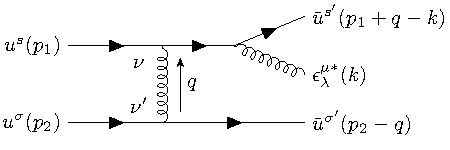
\includegraphics[width=.5\textwidth]{Large-Q-q2qg-A.pdf}\\
\vspace{1em}
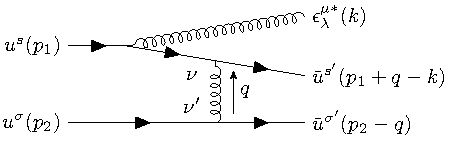
\includegraphics[width=.49\textwidth]{Large-Q-q2qg-B.pdf}\hfill
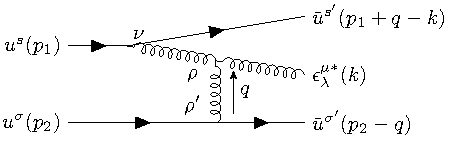
\includegraphics[width=.49\textwidth]{Large-Q-q2qg-C.pdf}
\caption{Three diagrams $A$ (Top), $B$ (Bottom left), $C$ (Bottom right) that contribute to the large angle scattering induced a quark splitting into a quark and a gluon in the forward region of the center-of-mass frame.}
\label{fig:feyn-q2qg}
\end{figure}

The Feynman diagrams to be included for $q+q\rightarrow q+g+q$ are shown in Figure \ref{fig:feyn-q2qg}.
The calculation uses exactly the same technique we used for the gluon splitting channel, and we present the result directly,
\begin{eqnarray}
\overline{|M^2|}_{g+q\rightarrow g+g+q} &=& 
 g^4 \frac{C_F}{d_F}\frac{4s^2}{q_\perp^4}x(1-x) \\\nonumber
&\times&g^2\frac{1+(1-x)^2}{x}  
\left(C_F\vec{A}^2 + C_F\vec{B}^2 - \left(2C_F-C_A\right)\vec{A}\cdot\vec{B}\right)\\
\vec{A} &=& \frac{\vec{k}_\perp - \vec{q}_\perp}{(\vec{k}_\perp - \vec{q}_\perp)^2} -  \frac{\vec{k}_\perp - x\vec{q}_\perp}{(\vec{k}_\perp - x\vec{q}_\perp)^2} \\
\vec{B} &=& \frac{\vec{k}_\perp - \vec{q}_\perp}{(\vec{k}_\perp - \vec{q}_\perp)^2} -  \frac{\vec{k}_\perp}{\vec{k}_\perp^2}
\end{eqnarray}


\paragraph*{Gluon splitting to two gluons}
\begin{figure}
\centering
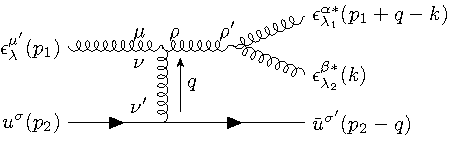
\includegraphics[width=.5\textwidth]{Large-Q-g2gg-A.pdf}\\
\vspace{1em}
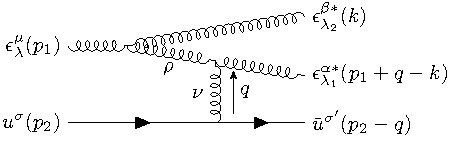
\includegraphics[width=.49\textwidth]{Large-Q-g2gg-B.pdf}\hfill
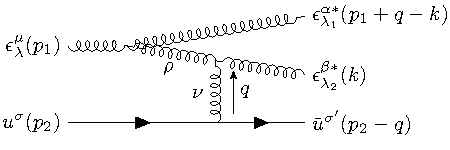
\includegraphics[width=.49\textwidth]{Large-Q-g2gg-C.pdf}
\caption{Three diagrams $A$ (Top), $B$ (Bottom left), $C$ (Bottom right) that contribute to the large angle scattering induced gluon splitting into two gluons in the forward region of the center-of-mass frame.}
\label{fig:feyn-g2gg}
\end{figure}

Finally, for $g+q\rightarrow g+q+g$, the Feynman diagrams are shown in Figure \ref{fig:feyn-g2gg}. 
The simplification of the two body collision amplitude can be done in a similar manner as the previous two channels. 
We only write down the splitting amplitude $g\rightarrow g+ g$ in detail.
Suppressing the color index, we label the initial gluon with $\epsilon_1^\mu(p)$, and the two daughter gluons with $\epsilon_2^\nu(k)$ and $\epsilon_3^\rho(q)$.
The splitting amplitudes are then (omitting the factor $-gf^{abc}$)
\begin{eqnarray}
iP &=& \epsilon^\mu_1\epsilon^\nu_2\epsilon^\rho_3
\left[
g_{\mu\nu} (p+k)_{\rho} +  g_{\nu\rho} (p+k)_{\mu} + g_{\rho\mu} (-q-p)_{\nu}
\right]\\
&=& -\vec{\epsilon}_{1,\perp}\cdot \vec{\epsilon}_{2,\perp} \left[(p+k)^+\frac{\vec{\epsilon}_{3,\perp}\cdot \vec{q}_\perp}{q^+} - \vec{\epsilon}_{3,\perp}\cdot (\vec{p}_\perp+\vec{k}_\perp)\right] \\\nonumber
&&-\vec{\epsilon}_{2,\perp}\cdot \vec{\epsilon}_{3,\perp} \left[(-k+q)^+\frac{\vec{\epsilon}_{1,\perp}\cdot \vec{p}_\perp}{p^+} - \vec{\epsilon}_{1,\perp}\cdot (-\vec{k}_\perp+\vec{q}_\perp)\right]
\\\nonumber
&&-\vec{\epsilon}_{3,\perp}\cdot \vec{\epsilon}_{1,\perp} \left[(-q-p)^+\frac{\vec{\epsilon}_{2,\perp}\cdot \vec{k}_\perp}{k^+} - \vec{\epsilon}_{2,\perp}\cdot (-\vec{q}_\perp-\vec{p}_\perp)\right]
\end{eqnarray}
There are four possible combinations of the polarization vectors, and their respective amplitude is computed as,
\begin{eqnarray}
iP = \sqrt{2}\left[x\vec{q}_\perp - (1-x)\vec{k}_\perp\right]\times 
\begin{cases}
\frac{1-x+x^2}{x(1-x)}, \hfill \lambda_1=\lambda_2=\lambda_3\\
-1, \hfill \lambda_1\neq\lambda_2=\lambda_3 \\
\frac{1}{x}, \hfill \lambda_1=\lambda_3\neq\lambda_2\\
\frac{1}{1-x}, \hfill \lambda_1=\lambda_2\neq\lambda_3
\end{cases}
\end{eqnarray}
Summing over the squared amplitude of all four cases and average over the initial gluon polarization, one gets the desired leading order QCD splitting function,
\begin{eqnarray}
2\frac{1+x^2+(1-x)^4}{x^2(1-x)^2} \left[x\vec{q}_\perp - (1-x)\vec{k}_\perp\right]^2.
\end{eqnarray}

Substitute the the amplitude in each diagram, the final squared matrix-element is 
\begin{eqnarray}
\overline{|M^2|}_{g+q\rightarrow g+g+q} &=&
g^4 \frac{C_A}{d_F}\frac{4s^2x(1-x)}{q_\perp^4} \\\nonumber
&\times&g^2\frac{1+x^4+(1-x)^4}{x(1-x)}   
\left(C_A\vec{A}^2 + C_A\vec{B}^2 - C_A\vec{A}\cdot\vec{B}\right)\\
\vec{A} &=& \frac{\vec{k}_\perp - x\vec{q}_\perp}{(\vec{k}_\perp - x\vec{q}_\perp)^2} -  \frac{\vec{k}_\perp - \vec{q}_\perp}{(\vec{k}_\perp - \vec{q}_\perp)^2} \\
\vec{B} &=& \frac{\vec{k}_\perp - x\vec{q}_\perp}{(\vec{k}_\perp - x\vec{q}_\perp)^2} -  \frac{\vec{k}_\perp}{\vec{k}_\perp^2}
\end{eqnarray}

\paragraph{Regulating the $2\rightarrow 3$ squared matrix-elements}
The divergence in the $q$ integration is removed by the requirement that this few-body matrix-element only applies to processes with $q>Q_{\textrm{cut}}$.
The collinear divergence when $k$ approaching $q$, $xq$ is regulated by including a gluon thermal mass. 
In practice, these collinear region will be further suppressed by the LPM effect.
The cross-section is obtained by integrating over the final state phase-space, where we have chosen to parameterize the three particle final state in terms of $k_\perp^2$, the rapidity of $k$ in the center-of-mass frame $y_k$, and the solid angle of the recoil medium particle.

\paragraph{Soft limit: the Gunion-Bertsch approximation}
The result we obtained for the $g\rightarrow g+g$ and $q\rightarrow q+g$ channel has a soft limit that goes back to the well known Gunion-Bertsch form. 
By soft limit, we require the radiated gluon energy to be small enough such that $xq_\perp \ll k_\perp$.
Then, the splitting amplitudes for both $g\rightarrow g+g$ and  $q\rightarrow q+g$ are simplified into the same form,
\begin{eqnarray}
\overline{|M|}^2_{22} x(1-x)g^2 \frac{2(1-x+O(x^2))}{x} C_A \left(\frac{\vec{k}_\perp}{k_\perp^2}-\frac{\vec{k}_\perp-\vec{q}_\perp}{(\vec{k}_\perp-\vec{q}_\perp)^2}\right)^2
\end{eqnarray}
Neglecting the $O(x^2)$ terms in the splitting function, the result is the same as the improved verison of the Gunion-Bertsch cross-section \cite{Fochler:2013epa} used in the full Boltzmann partonic transport model BAMPS \cite{Xu:2004mz},
\begin{eqnarray}
\overline{|M|}^2_{22} 8\pi C_A\alpha_s (1-x)^2 \left(\frac{\vec{k}_\perp}{k_\perp^2}-\frac{\vec{k}_\perp-\vec{q}_\perp}{(\vec{k}_\perp-\vec{q}_\perp)^2}\right)^2
\end{eqnarray}

\paragraph{The backward ($y_k < 0$) region}
We have mentioned in the beginning of the derivation that the condition $k_\perp^2 < x(1-x)\hat{s}$ restricts the splitting to be happen only for the parton moving in the $+z$ direction in the center-of-mass frame ($y_k > 0$).
For splitting that happens in the backward region, another set of diagrams contributes, where the splitting comes from the parton that moves in the $-z$ direction in the center-of-mass frame.
Also one needs a different gauge $A^- = 0$.
The derivation is similar to the previous ones, but with the definition of $x$ and $q$ changed to $x = k^-/\sqrt{s}$, and $q = p_1-p_3$.

To combine the results that is obtained in different regions of phase space ($y_k > 0$ and $y_k < 0$), we follow \cite{Fochler:2013epa} and defines,
\begin{eqnarray}
\bar{x} &=& \frac{(k + |k_z|)}{\sqrt{s}} = \frac{k_\perp e^{|y_k|}}{\sqrt{s}}\\ 
\bar{q} &=& \Theta(y_k)(p_2-p_4) + \Theta(-y_k)(p_1-p_3)
\end{eqnarray}
which replaces the original $x$ and $q$ in our formula, and the resultant matrix-elements can be used for both forward and backward regions.

\paragraph*{Relation to the Bethe-Heitler limit of the AMY formalisim}
Now we show the connection between the $2\rightarrow 3$ cross section obtained here and the Bethe-Heitler limit of the AMY equation.
In the Bethe-Heitler limit, the AMY integral equation can be solved approximately by treating $1/\tau_f$ as the leading factor. 
One get the splitting rate for each different channels (denoting $\vec{a}/a^2$ as $\vec{\phi}_{a}$), 
\begin{eqnarray}
R_{q\rightarrow q+g}^{BH} &\propto& g^2 P_{qg}^{q(0)}(x) \int d k^2 d q^2 \mathcal{A}(q^2) \left\{
C_A\vec{\phi}_k\cdot\left(\vec{\phi}_k-\vec{\phi}_{k-q}\right) \right.\\\nonumber
&&+\left. (2C_F-C_A) \vec{\phi}_k\cdot\left(\vec{\phi}_k-\vec{\phi}_{k+xq}\right)
+ C_A \vec{\phi}_k\cdot\left(\vec{\phi}_k - \vec{\phi}_{k+(1-x)q}\right)
\right\}
\\
R_{g\rightarrow g+g}^{BH} &\propto& g^2 P_{gg}^{g(0)}(x) \int d k^2 d q^2 \mathcal{A}(q^2) \left\{
C_A\vec{\phi}_k\cdot\left(\vec{\phi}_k-\vec{\phi}_{k-q}\right) \right.\\\nonumber
&&+\left. C_A \vec{\phi}_k\cdot\left(\vec{\phi}_k-\vec{\phi}_{k+xq}\right)
+ C_A \vec{\phi}_k\cdot\left(\vec{\phi}_k - \vec{\phi}_{k+(1-x)q}\right)
\right\}
\\
R_{g\rightarrow q+\bar{q}}^{BH} &\propto& g^2 P_{q\bar{q}}^{g(0)}(x) \int d k^2  d q^2 \mathcal{A}(q^2) \left\{
(2C_F-C_A)\vec{\phi}_k\cdot\left(\vec{\phi}_k-\vec{\phi}_{k-q}\right) \right.\\\nonumber
&&+\left. C_A \vec{\phi}_k\cdot\left(\vec{\phi}_k-\vec{\phi}_{k+xq}\right)
+ C_A \vec{\phi}_k\cdot\left(\vec{\phi}_k - \vec{\phi}_{k+(1-x)q}\right)
\right\}
\end{eqnarray}
with the collision kernel $\mathcal{A} = g^2 T m_D^2/q^2(q^2+m_D^2)$. These expression looks drastically different from the incoherent rate computed using the cross-section derived in the previous section, however, we would like to show that they are the same once integration over $dk^2$ is performed.
Therefore, the incoherent rate we used in the Boltzmann equation indeed recover the Bethe-Heitler limit of the AMY integral equation.

To show this, we start from the $2\rightarrow 3$ rate formula using the matrix-elements from equation. 
Starting from the $q\rightarrow q+g$ channel, the rate in our Boltzmann equation is,
\begin{eqnarray}
R_{q\rightarrow q+g} &\propto& g^2 P_{qg}^{q(0)}(x) \int  \frac{f(p_2)dp_2^3}{2E_2(2\pi)^3} d q^2 \frac{g^4}{q^4}\\\nonumber
&&  \int d k^2\left\{
C_F\left( \vec{\phi}_{k-q}-\vec{\phi}_{k-xq} \right)^2
+ C_F\left( \vec{\phi}_{k-q}-\vec{\phi}_{k} \right)^2\right.\\\nonumber
&&\left.
- (2C_F-C_A)\left( \vec{\phi}_{k-q}-\vec{\phi}_{k-xq} \right)\cdot \left( \vec{\phi}_{k-q}-\vec{\phi}_{k} \right)
\right\}
\end{eqnarray}
Focusing on the three products (squares) of $\vec{\phi}$s under the $dk^2$ integration, we are going to expand the first term in each product and then shift the argument of the first $\vec{\phi}$ to $k$, 
\begin{eqnarray}
R_{q\rightarrow q+g} &\propto& g^2 P_{qg}^{q(0)}(x) \int  \frac{f(p_2)dp_2^3}{2E_2(2\pi)^3} d q^2 \frac{g^4}{q^4}\\\nonumber
&&  \int d k^2\left\{
C_F\vec{\phi}_{k}\left( \vec{\phi}_{k}-\vec{\phi}_{k+(1-x)q} \right)
- C_F\vec{\phi}_{k}\left( \vec{\phi}_{k-(1-x)q}-\vec{\phi}_{k} \right)\right.
\\\nonumber
&&+ C_F\vec{\phi}_{k}\left( \vec{\phi}_{k}-\vec{\phi}_{k+q} \right)
- C_F\vec{\phi}_{k}\left( \vec{\phi}_{k-q}-\vec{\phi}_{k} \right)
\\\nonumber
&&\left.
- (2C_F-C_A)\vec{\phi}_{k}\cdot \left( \vec{\phi}_{k}-\vec{\phi}_{k+q} \right)
+(2C_F-C_A)\vec{\phi}_{k} \cdot \left( \vec{\phi}_{k-(1-x)q}-\vec{\phi}_{k+xq} \right)
\right\}
\end{eqnarray}
Next, flip  the sign of $q$ under the integration,
and meanwhile, insert a $-\vec{\phi}_k +\vec{\phi}_k$ in the brackets of the last term,
\begin{eqnarray}
R_{q\rightarrow q+g} &\propto& g^2 P_{qg}^{q(0)}(x) \int  \frac{f(p_2)dp_2^3}{2E_2(2\pi)^3} d q^2 \frac{g^4}{q^4}\\\nonumber
&&  \int d k^2\left\{
2C_F\vec{\phi}_{k}\left( \vec{\phi}_{k}-\vec{\phi}_{k+(1-x)q} \right)
+ 2C_F\vec{\phi}_{k}\left( \vec{\phi}_{k}-\vec{\phi}_{k+q} \right)
\right.
\\\nonumber
&&
- (2C_F-C_A)\vec{\phi}_{k}\cdot \left( \vec{\phi}_{k}-\vec{\phi}_{k+q} \right)
+(2C_F-C_A)\vec{\phi}_{k} \cdot \left( \vec{\phi}_{k+(1-x)q} -\vec{\phi}_k \right) \\\nonumber
&&\left.+(2C_F-C_A)\vec{\phi}_{k} \cdot \left(\vec{\phi}_k-\vec{\phi}_{k+xq} \right)
\right\}
\end{eqnarray}
After this manipulation, the first (second) term cancels the $C_F$ part of the fourth (third) term, 
\begin{eqnarray}
R_{q\rightarrow q+g} &\propto& g^2 P_{qg}^{q(0)}(x) \int  \frac{f(p_2)dp_2^3}{2E_2(2\pi)^3} d q^2 \frac{g^4}{q^4}\\\nonumber
&&  \int d k^2\left\{
C_A\vec{\phi}_{k}\cdot \left( \vec{\phi}_{k}-\vec{\phi}_{k+q} \right)
+C_A\vec{\phi}_{k} \cdot \left( \vec{\phi}_k - \vec{\phi}_{k+(1-x)q}\right) \right.\\\nonumber
&&\left.+(2C_F-C_A)\vec{\phi}_{k} \cdot \left(\vec{\phi}_k-\vec{\phi}_{k+xq} \right)
\right\}
\end{eqnarray}
which is the same integration as the one obtained from the Bethe-Heitler limit of the AMY equation (neglecting the screen mass in $\mathcal{A}$ when $q^2 \gg m_D^2$)
The equivalence between these two expressions of the $g\rightarrow g+g$ channel and the $g\rightarrow q+\bar{q}$ channel can also be shown similarly.

\paragraph*{Mass effect in the $2\rightarrow 3$ squared matrix-elements}
For completeness, we briefly outline the derivation of $2\rightarrow 3$ cross-section with mass effect.
As a remark, putting heavy flavor mass directly into the these matrix-elements are certainly legitimate if one only focus on $2\rightarrow 3$ processes.
But once we want to approximate the effect of multiple scatterings:
$(n \rightarrow n+1) \approx (2 \rightarrow 3)(2 \rightarrow 2)\cdots(2 \rightarrow 2)\times \textrm{corrections}$, it is not advantages to put the mass effect into the $(2 \rightarrow 3)$ part, but into the last step of corrections, which is the approach we used.


First, we still work under the assumption that $M \ll E$, and will only keep terms when $M$ is making direct comparison to $k_\perp, q_\perp$.
The kinematics are now changed to,
\begin{eqnarray}
p_1 &=& (\sqrt{s}, 0, \vec{0})\\
p_2 &=& (0, \sqrt{s}, \vec{0})\\
k &=& (x\sqrt{s}, \frac{k_\perp^2}{x\sqrt{s}}, \vec{k}_\perp)\\
q &\sim& (-\frac{q_\perp^2\sqrt{s}}{s-M^2}, \frac{x(\vec{q}_\perp-\vec{k}_\perp)^2 + (1-x)k_\perp^2 + x^2M^2}{x(1-x)\sqrt{s}}, \vec{k}_\perp)
\end{eqnarray}
For the splitting amplitude, off diagonal elements of $\epsilon_{\lambda, \mu}(c) \bar{u}_s(a) \gamma^\mu v_{s'} (b)$ also needs to be included for helicity flipping process. 
Moreover,
\begin{eqnarray}
\sqrt{p\cdot \sigma} &=& \frac{p\cdot \sigma + M}{\sqrt{2(E+M)}} \approx \frac{p\cdot \sigma + M}{\sqrt{2E}} \\
\sqrt{p\cdot \bar{\sigma}} &=& \frac{p\cdot \bar{\sigma} + M}{\sqrt{2(E+M)}} \approx \frac{p\cdot \bar{\sigma} + M}{\sqrt{2E}}
\end{eqnarray}
where we have omitted the mass in the denominator since it only involves corrections of order $M/E$.
From this one can see that the previous calculation can be used for the massive case with the substitution  $a^\pm \rightarrow a^\pm +M$ and $b^\pm \rightarrow b^\pm +M$.
Then, the splitting amplitude becomes,
\begin{eqnarray}
\epsilon_{\lambda, \mu} \bar{u}_s(a)\gamma^\mu v_{s'}(b)&=& \frac{1}{\sqrt{2ab}}
\xi_s^T A_{ss'} \eta_{s'}\\
A_{\uparrow\uparrow} &=&
\delta_{\lambda L} 2b_z a^\perp_L + \delta_{\lambda R} 2a_z b^\perp_R + \frac{c^\perp_\lambda}{c^+} (a^\perp_L b^\perp_R - a^+ b^+) \\
A_{\downarrow\downarrow} &=&
-\delta_{\lambda L}2a_z b^\perp_L - \delta_{\lambda R}2b_z a^\perp_R - \frac{c^\perp_\lambda}{c^+} (a^\perp_R b^\perp_L - a^+ b^+) \\
A_{\uparrow\downarrow} &=&
\delta_{\lambda L} 2a^\perp_L b^\perp_L + \delta_{\lambda R} (a^+b^-+a^-b^+) - \frac{c^\perp_\lambda}{c^+} (a^+b^\perp + a^\perp b^+) \\
A_{\downarrow\uparrow} &=&
 \delta_{\lambda L} (a^+b^-+a^-b^+) + \delta_{\lambda L} 2a^\perp_R b^\perp_R - \frac{c^\perp_\lambda}{c^+} (a^+b^\perp + a^\perp b^+) 
\end{eqnarray}

